\documentclass{beamer}
\usepackage[utf8]{inputenc}
\usepackage{verbatim}
\usepackage{ulem}
\usepackage{fancyvrb}
\usepackage{color}
\usepackage{tikz}

\makeatletter
\def\PY@reset{\let\PY@it=\relax \let\PY@bf=\relax%
    \let\PY@ul=\relax \let\PY@tc=\relax%
    \let\PY@bc=\relax \let\PY@ff=\relax}
\def\PY@tok#1{\csname PY@tok@#1\endcsname}
\def\PY@toks#1+{\ifx\relax#1\empty\else%
    \PY@tok{#1}\expandafter\PY@toks\fi}
\def\PY@do#1{\PY@bc{\PY@tc{\PY@ul{%
    \PY@it{\PY@bf{\PY@ff{#1}}}}}}}
\def\PY#1#2{\PY@reset\PY@toks#1+\relax+\PY@do{#2}}

\expandafter\def\csname PY@tok@gd\endcsname{\def\PY@tc##1{\textcolor[rgb]{0.63,0.00,0.00}{##1}}}
\expandafter\def\csname PY@tok@gu\endcsname{\let\PY@bf=\textbf\def\PY@tc##1{\textcolor[rgb]{0.50,0.00,0.50}{##1}}}
\expandafter\def\csname PY@tok@gt\endcsname{\def\PY@tc##1{\textcolor[rgb]{0.00,0.25,0.82}{##1}}}
\expandafter\def\csname PY@tok@gs\endcsname{\let\PY@bf=\textbf}
\expandafter\def\csname PY@tok@gr\endcsname{\def\PY@tc##1{\textcolor[rgb]{1.00,0.00,0.00}{##1}}}
\expandafter\def\csname PY@tok@cm\endcsname{\let\PY@it=\textit\def\PY@tc##1{\textcolor[rgb]{0.25,0.50,0.50}{##1}}}
\expandafter\def\csname PY@tok@vg\endcsname{\def\PY@tc##1{\textcolor[rgb]{0.10,0.09,0.49}{##1}}}
\expandafter\def\csname PY@tok@m\endcsname{\def\PY@tc##1{\textcolor[rgb]{0.40,0.40,0.40}{##1}}}
\expandafter\def\csname PY@tok@mh\endcsname{\def\PY@tc##1{\textcolor[rgb]{0.40,0.40,0.40}{##1}}}
\expandafter\def\csname PY@tok@go\endcsname{\def\PY@tc##1{\textcolor[rgb]{0.50,0.50,0.50}{##1}}}
\expandafter\def\csname PY@tok@ge\endcsname{\let\PY@it=\textit}
\expandafter\def\csname PY@tok@vc\endcsname{\def\PY@tc##1{\textcolor[rgb]{0.10,0.09,0.49}{##1}}}
\expandafter\def\csname PY@tok@il\endcsname{\def\PY@tc##1{\textcolor[rgb]{0.40,0.40,0.40}{##1}}}
\expandafter\def\csname PY@tok@cs\endcsname{\let\PY@it=\textit\def\PY@tc##1{\textcolor[rgb]{0.25,0.50,0.50}{##1}}}
\expandafter\def\csname PY@tok@cp\endcsname{\def\PY@tc##1{\textcolor[rgb]{0.74,0.48,0.00}{##1}}}
\expandafter\def\csname PY@tok@gi\endcsname{\def\PY@tc##1{\textcolor[rgb]{0.00,0.63,0.00}{##1}}}
\expandafter\def\csname PY@tok@gh\endcsname{\let\PY@bf=\textbf\def\PY@tc##1{\textcolor[rgb]{0.00,0.00,0.50}{##1}}}
\expandafter\def\csname PY@tok@ni\endcsname{\let\PY@bf=\textbf\def\PY@tc##1{\textcolor[rgb]{0.60,0.60,0.60}{##1}}}
\expandafter\def\csname PY@tok@nl\endcsname{\def\PY@tc##1{\textcolor[rgb]{0.63,0.63,0.00}{##1}}}
\expandafter\def\csname PY@tok@nn\endcsname{\let\PY@bf=\textbf\def\PY@tc##1{\textcolor[rgb]{0.00,0.00,1.00}{##1}}}
\expandafter\def\csname PY@tok@no\endcsname{\def\PY@tc##1{\textcolor[rgb]{0.53,0.00,0.00}{##1}}}
\expandafter\def\csname PY@tok@na\endcsname{\def\PY@tc##1{\textcolor[rgb]{0.49,0.56,0.16}{##1}}}
\expandafter\def\csname PY@tok@nb\endcsname{\def\PY@tc##1{\textcolor[rgb]{0.00,0.50,0.00}{##1}}}
\expandafter\def\csname PY@tok@nc\endcsname{\let\PY@bf=\textbf\def\PY@tc##1{\textcolor[rgb]{0.00,0.00,1.00}{##1}}}
\expandafter\def\csname PY@tok@nd\endcsname{\def\PY@tc##1{\textcolor[rgb]{0.67,0.13,1.00}{##1}}}
\expandafter\def\csname PY@tok@ne\endcsname{\let\PY@bf=\textbf\def\PY@tc##1{\textcolor[rgb]{0.82,0.25,0.23}{##1}}}
\expandafter\def\csname PY@tok@nf\endcsname{\def\PY@tc##1{\textcolor[rgb]{0.00,0.00,1.00}{##1}}}
\expandafter\def\csname PY@tok@si\endcsname{\let\PY@bf=\textbf\def\PY@tc##1{\textcolor[rgb]{0.73,0.40,0.53}{##1}}}
\expandafter\def\csname PY@tok@s2\endcsname{\def\PY@tc##1{\textcolor[rgb]{0.73,0.13,0.13}{##1}}}
\expandafter\def\csname PY@tok@vi\endcsname{\def\PY@tc##1{\textcolor[rgb]{0.10,0.09,0.49}{##1}}}
\expandafter\def\csname PY@tok@nt\endcsname{\let\PY@bf=\textbf\def\PY@tc##1{\textcolor[rgb]{0.00,0.50,0.00}{##1}}}
\expandafter\def\csname PY@tok@nv\endcsname{\def\PY@tc##1{\textcolor[rgb]{0.10,0.09,0.49}{##1}}}
\expandafter\def\csname PY@tok@s1\endcsname{\def\PY@tc##1{\textcolor[rgb]{0.73,0.13,0.13}{##1}}}
\expandafter\def\csname PY@tok@sh\endcsname{\def\PY@tc##1{\textcolor[rgb]{0.73,0.13,0.13}{##1}}}
\expandafter\def\csname PY@tok@sc\endcsname{\def\PY@tc##1{\textcolor[rgb]{0.73,0.13,0.13}{##1}}}
\expandafter\def\csname PY@tok@sx\endcsname{\def\PY@tc##1{\textcolor[rgb]{0.00,0.50,0.00}{##1}}}
\expandafter\def\csname PY@tok@bp\endcsname{\def\PY@tc##1{\textcolor[rgb]{0.00,0.50,0.00}{##1}}}
\expandafter\def\csname PY@tok@c1\endcsname{\let\PY@it=\textit\def\PY@tc##1{\textcolor[rgb]{0.25,0.50,0.50}{##1}}}
\expandafter\def\csname PY@tok@kc\endcsname{\let\PY@bf=\textbf\def\PY@tc##1{\textcolor[rgb]{0.00,0.50,0.00}{##1}}}
\expandafter\def\csname PY@tok@c\endcsname{\let\PY@it=\textit\def\PY@tc##1{\textcolor[rgb]{0.25,0.50,0.50}{##1}}}
\expandafter\def\csname PY@tok@mf\endcsname{\def\PY@tc##1{\textcolor[rgb]{0.40,0.40,0.40}{##1}}}
\expandafter\def\csname PY@tok@err\endcsname{\def\PY@bc##1{\setlength{\fboxsep}{0pt}\fcolorbox[rgb]{1.00,0.00,0.00}{1,1,1}{\strut ##1}}}
\expandafter\def\csname PY@tok@kd\endcsname{\let\PY@bf=\textbf\def\PY@tc##1{\textcolor[rgb]{0.00,0.50,0.00}{##1}}}
\expandafter\def\csname PY@tok@ss\endcsname{\def\PY@tc##1{\textcolor[rgb]{0.10,0.09,0.49}{##1}}}
\expandafter\def\csname PY@tok@sr\endcsname{\def\PY@tc##1{\textcolor[rgb]{0.73,0.40,0.53}{##1}}}
\expandafter\def\csname PY@tok@mo\endcsname{\def\PY@tc##1{\textcolor[rgb]{0.40,0.40,0.40}{##1}}}
\expandafter\def\csname PY@tok@kn\endcsname{\let\PY@bf=\textbf\def\PY@tc##1{\textcolor[rgb]{0.00,0.50,0.00}{##1}}}
\expandafter\def\csname PY@tok@mi\endcsname{\def\PY@tc##1{\textcolor[rgb]{0.40,0.40,0.40}{##1}}}
\expandafter\def\csname PY@tok@gp\endcsname{\let\PY@bf=\textbf\def\PY@tc##1{\textcolor[rgb]{0.00,0.00,0.50}{##1}}}
\expandafter\def\csname PY@tok@o\endcsname{\def\PY@tc##1{\textcolor[rgb]{0.40,0.40,0.40}{##1}}}
\expandafter\def\csname PY@tok@kr\endcsname{\let\PY@bf=\textbf\def\PY@tc##1{\textcolor[rgb]{0.00,0.50,0.00}{##1}}}
\expandafter\def\csname PY@tok@s\endcsname{\def\PY@tc##1{\textcolor[rgb]{0.73,0.13,0.13}{##1}}}
\expandafter\def\csname PY@tok@kp\endcsname{\def\PY@tc##1{\textcolor[rgb]{0.00,0.50,0.00}{##1}}}
\expandafter\def\csname PY@tok@w\endcsname{\def\PY@tc##1{\textcolor[rgb]{0.73,0.73,0.73}{##1}}}
\expandafter\def\csname PY@tok@kt\endcsname{\def\PY@tc##1{\textcolor[rgb]{0.69,0.00,0.25}{##1}}}
\expandafter\def\csname PY@tok@ow\endcsname{\let\PY@bf=\textbf\def\PY@tc##1{\textcolor[rgb]{0.67,0.13,1.00}{##1}}}
\expandafter\def\csname PY@tok@sb\endcsname{\def\PY@tc##1{\textcolor[rgb]{0.73,0.13,0.13}{##1}}}
\expandafter\def\csname PY@tok@k\endcsname{\let\PY@bf=\textbf\def\PY@tc##1{\textcolor[rgb]{0.00,0.50,0.00}{##1}}}
\expandafter\def\csname PY@tok@se\endcsname{\let\PY@bf=\textbf\def\PY@tc##1{\textcolor[rgb]{0.73,0.40,0.13}{##1}}}
\expandafter\def\csname PY@tok@sd\endcsname{\let\PY@it=\textit\def\PY@tc##1{\textcolor[rgb]{0.73,0.13,0.13}{##1}}}

\def\PYZbs{\char`\\}
\def\PYZus{\char`\_}
\def\PYZob{\char`\{}
\def\PYZcb{\char`\}}
\def\PYZca{\char`\^}
\def\PYZam{\char`\&}
\def\PYZlt{\char`\<}
\def\PYZgt{\char`\>}
\def\PYZsh{\char`\#}
\def\PYZpc{\char`\%}
\def\PYZdl{\char`\$}
\def\PYZti{\char`\~}
% for compatibility with earlier versions
\def\PYZat{@}
\def\PYZlb{[}
\def\PYZrb{]}
\makeatother

%\usetheme{default}
\begin{document}
\title{Workshop Django}
\author{Laurent Peuch}

\maketitle{}

\begin{frame}{Plan}
    \begin{itemize}
        \item Installation
        \item Hello world
        \item MTV basique
        \item Avancé
        \item Jquery
    \end{itemize}
\end{frame}

\begin{frame}{Objectif}
\begin{itemize}
    \item vous apprendre la base de Django et la structure classique d'un projet Django
    \item vous donner une vision d'ensemble de ce qui est possible/disponible
    \item pour pouvoir continuer à apprendre la suite par vous même
    \item que ces slides puissent être un support pour vous
    \item plus ou moins vous donner ce qu'il faut pour bosser sur la partie Django de p402
\end{itemize}
\end{frame}

\begin{frame}{Requirements}
\begin{itemize}
    \item savoir coder
    \item connaitre la programmation orienté objet
    \item python (la base)
    \item sql (pas forcement poussée)
    \item html (la base)
    \item regexp (la base)
    \item savoir utiliser un shell (la base)
\end{itemize}
\end{frame}

\begin{frame}[fragile]{}
    \LARGE \begin{center}https://djangoproject.com\end{center}
\end{frame}

\begin{frame}{Introduction}
    \vspace{3mm}
    C'est quoi Django ?
    \begin{itemize}
        \item framework web en python\pause
        \item full stacked (vs microframework comme flask, bottle et les 15 milles autres)\pause
        \item vous "impose" un orm et un système de templates (changeable tous les 2 mais pas pensé pour)\pause
        \item mais en échange vous avez les Django app\pause
        \item facile à utiliser (quasi tout), gros gain de productivité mais beaucoup à apprendre, vous allez souvent utiliser la documentation
    \end{itemize}
\end{frame}

\begin{frame}[fragile]{}
\begin{LARGE}
\begin{center}
Installation
\end{center}
\end{LARGE}
\end{frame}

\begin{frame}{Installation}
2 façons de faire
\begin{itemize}
    \item la classique avec le pkg manager de la distribution (eg: sudo apt-get install django)
    \item en utilisant pypi via pip (on va utiliser celle là) dans un virtualenv
\end{itemize}
\end{frame}

\begin{frame}{Installation}
    Faire:
    \begin{itemize}
        \item Installation de pip (sudo apt-get install python-pip)\pause
        \item sudo pip install virtualenv (ou alors avec le package python-virtualenv)\pause
        \item aller dans un nouveau répertoire (mkdir blog \&\& cd blog)\pause
        \item virtualenv - -no-site-packages - -distribute ve\pause
        \item source ve/bin/activate \# pour rentrer dans le venv\pause
        \item pip install django\pause
        \item rehash \# pour zsh
    \end{itemize}
    \vspace{3mm}
    \pause
    Si vous voulez sortir du venv:
    \begin{itemize}
        \item deactivate
    \end{itemize}
\end{frame}

\begin{frame}[fragile]{Mon premier projet Django}
    Faire dans le virtualenv:
            \begin{verbatim}
    django-admin.py startproject <nom du projet>
            \end{verbatim}
    \pause
    Lancer le serveur de développement:
    \begin{verbatim}
    cd <nom du projet> && python manage.py runserver
    \end{verbatim}
    Puis aller sur http://0.0.0.0:8000
\end{frame}

\begin{frame}[fragile]{Django 1.4}
    Vous allez obtenir une hiérarchie du style:

\begin{verbatim}
    project/urls.py
    project/settings.py
    project/__init__.py
    project/wsgi.py
    manage.py
\end{verbatim}

\end{frame}

\begin{frame}[fragile]{Django $\leq$ 1.3}
    Remarque: vous allez aussi rencontrer des projets ayant la forme suivante (Django $\leq$ 1.3)
    \begin{verbatim}
    urls.py
    settings.py
    manage.py
    __init__.py
    \end{verbatim}
\end{frame}

\begin{frame}[fragile]{}
\begin{LARGE}
\begin{center}
Hello World
\end{center}
\end{LARGE}
\end{frame}

\begin{frame}[fragile]{urls.py}
\begin{footnotesize}
\begin{Verbatim}[commandchars=\\\{\}]
\PY{k+kn}{from} \PY{n+nn}{django.conf.urls} \PY{k+kn}{import} \PY{n}{patterns}\PY{p}{,} \PY{n}{include}\PY{p}{,} \PY{n}{url}

\PY{c}{\PYZsh{} Uncomment the next two lines to enable the admin:}
\PY{c}{\PYZsh{} from django.contrib import admin}
\PY{c}{\PYZsh{} admin.autodiscover()}

\PY{n}{urlpatterns} \PY{o}{=} \PY{n}{patterns}\PY{p}{(}\PY{l+s}{'}\PY{l+s}{'}\PY{p}{,}
    \PY{c}{\PYZsh{} Examples:}
    \PY{c}{\PYZsh{} url(r'\PYZca{}\PYZdl{}', 'project.views.home', name='home'),}
    \PY{c}{\PYZsh{} url(r'\PYZca{}project/', include('project.foo.urls')),}

    \PY{c}{\PYZsh{} Uncomment the admin/doc line below to enable admin documentation:}
    \PY{c}{\PYZsh{} url(r'\PYZca{}admin/doc/', include('django.contrib.admindocs.urls')),}

    \PY{c}{\PYZsh{} Uncomment the next line to enable the admin:}
    \PY{c}{\PYZsh{} url(r'\PYZca{}admin/', include(admin.site.urls)),}
\PY{p}{)}
\end{Verbatim}
\end{footnotesize}
\end{frame}

\begin{frame}[fragile]{Hello World}
\begin{footnotesize}
\begin{Verbatim}[commandchars=\\\{\}]
\PY{k+kn}{from} \PY{n+nn}{django.conf.urls} \PY{k+kn}{import} \PY{n}{patterns}\PY{p}{,} \PY{n}{include}\PY{p}{,} \PY{n}{url}
\PY{k+kn}{from} \PY{n+nn}{django.http} \PY{k+kn}{import} \PY{n}{HttpResponse}

\PY{k}{def} \PY{n+nf}{hello}\PY{p}{(}\PY{n}{request}\PY{p}{)}\PY{p}{:}
    \PY{k}{return} \PY{n}{HttpResponse}\PY{p}{(}\PY{l+s}{"}\PY{l+s}{Hello World!}\PY{l+s}{"}\PY{p}{)}

\PY{n}{urlpatterns} \PY{o}{=} \PY{n}{patterns}\PY{p}{(}\PY{l+s}{'}\PY{l+s}{'}\PY{p}{,}
    \PY{n}{url}\PY{p}{(}\PY{l+s}{r'}\PY{l+s}{\PYZca{}\PYZdl{}}\PY{l+s}{'}\PY{p}{,} \PY{n}{hello}\PY{p}{)}\PY{p}{,}
\PY{p}{)}
\end{Verbatim}
\end{footnotesize}

Remarque: traditionnelement ces fonctions sont dans un fichier $views.py$

\end{frame}

\begin{frame}[fragile]{La vie d'une requète}

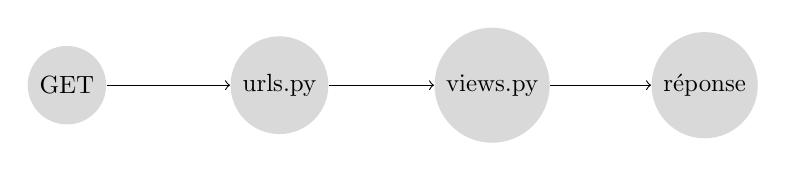
\begin{tikzpicture}[scale=.9, transform shape]
\tikzstyle{every node} = [circle, fill=gray!30]
\node (a) at (0, 0) {GET};
\node (b) at (3, 0) {urls.py};
\node (c) at (6, 0) {views.py};
\node (d) at (9, 0) {réponse};
\foreach \from/\to in {a/b, b/c, c/d}
\draw [->] (\from) -- (\to);
\end{tikzpicture}

\end{frame}

\begin{frame}[fragile]{}
\begin{LARGE}
\begin{center}
MTV
\end{center}
\end{LARGE}
\end{frame}

\begin{frame}[fragile]{MTV}

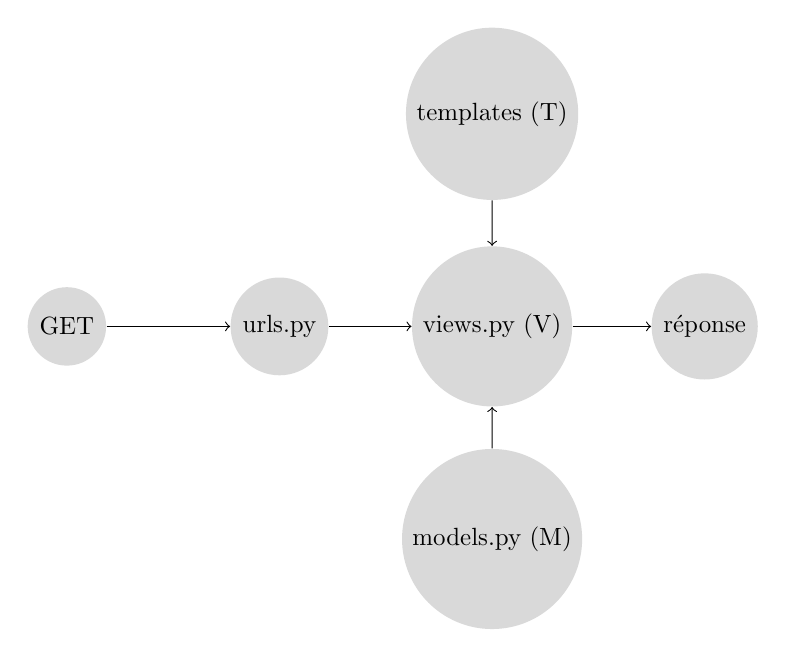
\begin{tikzpicture}[scale=.9, transform shape]
\tikzstyle{every node} = [circle, fill=gray!30]
\node (a) at (0, 0) {GET};
\node (b) at (3, 0) {urls.py};
\node (c) at (6, 0) {views.py (V)};
\node (e) at (6, 3) {templates (T)};
\node (f) at (6, -3) {models.py (M)};
\node (d) at (9, 0) {réponse};
\foreach \from/\to in {a/b, b/c, c/d, e/c, f/c}
\draw [->] (\from) -- (\to);
\end{tikzpicture}

\end{frame}

\begin{frame}[fragile]{Plan pour la partie mtv}
    \begin{itemize}
        \item templates
        \item models
        \item urls.py
        \item interface admin
    \end{itemize}
    Objectif: créer un mini blog (que sur la racine ($/$) s'affiche la liste de posts et sur $/<post\_id>/$ s'affiche un post).
\end{frame}

\begin{frame}[fragile]{}
\begin{LARGE}
\begin{center}
Templates
\end{center}
\end{LARGE}
\end{frame}

\begin{frame}[fragile]{Templates}
    Dans le répertoire de votre projet, au niveau où il y a le $manage.py$ faire:
    \begin{verbatim}
    mkdir templates
    \end{verbatim}
    Puis créer un fichier $templates/hello.html$ contenant:
    \begin{verbatim}
    <p>Hello {{ name }}</p>
    \end{verbatim}
\end{frame}

\begin{frame}[fragile]{Utiliser un template}
    Utiliser un template version moyen âge:

\begin{footnotesize}
\begin{Verbatim}[commandchars=\\\{\}]
\PY{k+kn}{from} \PY{n+nn}{django.template} \PY{k+kn}{import} \PY{n}{Context}\PY{p}{,} \PY{n}{loader}

\PY{k}{def} \PY{n+nf}{hello}\PY{p}{(}\PY{n}{request}\PY{p}{)}\PY{p}{:}
    \PY{n}{t} \PY{o}{=} \PY{n}{loader}\PY{o}{.}\PY{n}{get\PYZus{}template}\PY{p}{(}\PY{l+s}{'}\PY{l+s}{hello.html}\PY{l+s}{'}\PY{p}{)}
    \PY{n}{c} \PY{o}{=} \PY{n}{Context}\PY{p}{(}\PY{p}{\PYZob{}}
        \PY{l+s}{'}\PY{l+s}{name}\PY{l+s}{'}\PY{p}{:} \PY{l+s}{'argument'}\PY{p}{,}
    \PY{p}{\PYZcb{}}\PY{p}{)}
    \PY{k}{return} \PY{n}{HttpResponse}\PY{p}{(}\PY{n}{t}\PY{o}{.}\PY{n}{render}\PY{p}{(}\PY{n}{c}\PY{p}{)}\PY{p}{)}
\end{Verbatim}
\end{footnotesize}

On utilisera \bf{jamais}  ça.
\end{frame}

\begin{frame}[fragile]{Utiliser un template}
    Ce que tout le monde utilise:

\begin{footnotesize}
\begin{Verbatim}[commandchars=\\\{\}]
\PY{k+kn}{from} \PY{n+nn}{django.shortcuts} \PY{k+kn}{import} \PY{n}{render}

\PY{k}{def} \PY{n+nf}{hello}\PY{p}{(}\PY{n}{request}\PY{p}{)}\PY{p}{:}
    \PY{k}{return} \PY{n}{render}\PY{p}{(}\PY{n}{request}\PY{p}{,} \PY{l+s}{"}\PY{l+s}{hello.html}\PY{l+s}{"}\PY{p}{,} \PY{p}{\PYZob{}}\PY{l+s}{"}\PY{l+s}{name}\PY{l+s}{"}\PY{p}{:} \PY{l+s}{"}\PY{l+s}{World}\PY{l+s}{"}\PY{p}{\PYZcb{}}\PY{p}{)}
\end{Verbatim}
\end{footnotesize}

\end{frame}

\begin{frame}[fragile]{Utiliser un template}
    Si vous essayez d'aller sur $http://0.0.0.0:8000/$ vous allez avoir une erreur $TemplateDoesNotExist at /$.

    \vspace{3mm}

    C'est parce que Django demande qu'on lui dise où sont les templates (sauf pour les apps, cf plus tard).

    \vspace{3mm}

    Cela se fait dans le fichier $settings.py$.
\end{frame}

\begin{frame}[fragile]{Utiliser un template}
    Dans $settings.py$ chercher un truc qui ressemble à ça:

\begin{footnotesize}
    \begin{verbatim}
TEMPLATE_DIRS = (
    # Put strings here, like "/home/html/django_templates" or "C:/www/django/templates".
    # Always use forward slashes, even on Windows.
    # Don't forget to use absolute paths, not relative paths.
)
    \end{verbatim}
\end{footnotesize}\pause

Et mettre quelque chose du style:

\begin{footnotesize}
\begin{verbatim}
TEMPLATE_DIRS = (
    '/home/urlab/code/slides/workshop-django/1.4/project/templates',
)
\end{verbatim}
\end{footnotesize}\pause

Remarque: ce n'est pas portable, en vrai on utilise des paths relatifs, ici par simplicité je ne l'ai pas montré.\pause

\vspace{3mm}
\bf La virgule à la fin du string est OBLIGATOIRE sinon python ne considère pas que c'est un tuple (une liste à taille fixe).

\end{frame}

\begin{frame}[fragile]{Utiliser un template}
    Retourner sur $http://0.0.0.0:8000/$, cela devrait fonctionner désormait.

    Remarque: vérifier que le serveur de dev se lance bien et qu'il ne montre pas d'erreurs.
\end{frame}

\begin{frame}[fragile]{Syntaxe des templates}
    In a nutshell:

\begin{verbatim}
{{ nom_de_variable }} <- pour accèder à des variables

 <- pour le reste (les "templatetags")
\end{verbatim}

Volontairement simple, le but c'est de ne pas y avoir de logique. C'est pensé pour qu'un designer qui ne connaisse pas la programmation puisse s'en servir.
\end{frame}

\begin{frame}[fragile]{Syntaxe des templates}
Les appels aux attributs d'un objet pythons sont uniformisés, cela veut dire en gros que:
\begin{verbatim}
objet.attribut
objet.methode()
objet[clef]
\end{verbatim}
\vspace{10mm}
\end{frame}

\begin{frame}[fragile]{Syntaxe des templates}
Les appels aux attributs d'un objet pythons sont uniformisés, cela veut dire en gros que ... s'écrivent tous:
\begin{verbatim}
objet.attribut  -> {{ objet.attribut }}
objet.methode() -> {{ objet.methode }}
objet[clef]     -> {{ objet.clef }}
\end{verbatim}
\pause
Remarque: \bf on ne peut pas passer d'arguments à une méthode dans un template, il faut passer par des templatetags.
\end{frame}

\begin{frame}[fragile]{Syntaxe des templates}
    Une liste des templatetags de base:\pause
\begin{verbatim}

    ...

\end{verbatim}
\pause
\begin{verbatim}

    ...

    ...

\end{verbatim}
Les conditions sont très similaire à celles de python.
\end{frame}

\begin{frame}[fragile]{}
\begin{LARGE}
\begin{center}
ORM
\end{center}
\end{LARGE}
\end{frame}

\begin{frame}[fragile]{Modèles}
    On veut pouvoir stocker des données, ici on utilise une base de données SQL via l'ORM de Django.

    \vspace{3mm}
    (ORM == object-relationnal mapping, une abstraction de la base de données)
\end{frame}

\begin{frame}[fragile]{Mon premier modèle}

Exemple:
\begin{footnotesize}
\begin{Verbatim}[commandchars=\\\{\}]
\PY{k+kn}{from} \PY{n+nn}{django.db} \PY{k+kn}{import} \PY{n}{models}

\PY{k}{class} \PY{n+nc}{Post}\PY{p}{(}\PY{n}{models}\PY{o}{.}\PY{n}{Model}\PY{p}{)}\PY{p}{:}
    \PY{n}{title} \PY{o}{=} \PY{n}{models}\PY{o}{.}\PY{n}{CharField}\PY{p}{(}\PY{n}{max\PYZus{}length}\PY{o}{=}\PY{l+m+mi}{255}\PY{p}{)}
    \PY{n}{content} \PY{o}{=} \PY{n}{models}\PY{o}{.}\PY{n}{TextField}\PY{p}{(}\PY{p}{)}
\end{Verbatim}
\end{footnotesize}

À mettre dans $nom\_du\_projet/models.py$.

\vspace{3mm}
Remarque: ici c'est pour apprendre, en vrai ce fichier sera dans une app.

\vspace{3mm}
Autre remarque: si ce n'est pas spécifié Django créera une clef primaire pour vous qui s'appelera $id$ (et elle a un alias $pk$).

\end{frame}

\begin{frame}[fragile]{Créer la base de données}
    Maintenant qu'on a décrit un modèle, on doit demander à Django de le créer dans la base de données. Pour cela on doit faire la commande:

\begin{verbatim}
    python manage.py syncdb
\end{verbatim}

\pause
    Cela va produire une erreur, car on a pas dit à Django quelle base de données utiliser.
    \vspace{3mm}

    Cela se fait dans $settings.py$.
\end{frame}

\begin{frame}[fragile]{Configurer la base de donnée}
    Dans $settings.py$ changer:

\begin{footnotesize}
\begin{Verbatim}[commandchars=\\\{\}]
\PY{n}{DATABASES} \PY{o}{=} \PY{p}{\PYZob{}}
    \PY{l+s}{'}\PY{l+s}{default}\PY{l+s}{'}\PY{p}{:} \PY{p}{\PYZob{}}
        \PY{l+s}{'}\PY{l+s}{ENGINE}\PY{l+s}{'}\PY{p}{:} \PY{l+s}{'}\PY{l+s}{django.db.backends.}\PY{l+s}{'}\PY{p}{,} \PY{c}{\PYZsh{} Add 'postgresql\PYZus{}psycopg2', 'mysql', 'sqlite3' or 'oracle'.}
        \PY{l+s}{'}\PY{l+s}{NAME}\PY{l+s}{'}\PY{p}{:} \PY{l+s}{'}\PY{l+s}{'}\PY{p}{,}                      \PY{c}{\PYZsh{} Or path to database file if using sqlite3.}
        \PY{l+s}{'}\PY{l+s}{USER}\PY{l+s}{'}\PY{p}{:} \PY{l+s}{'}\PY{l+s}{'}\PY{p}{,}                      \PY{c}{\PYZsh{} Not used with sqlite3.}
        \PY{l+s}{'}\PY{l+s}{PASSWORD}\PY{l+s}{'}\PY{p}{:} \PY{l+s}{'}\PY{l+s}{'}\PY{p}{,}                  \PY{c}{\PYZsh{} Not used with sqlite3.}
        \PY{l+s}{'}\PY{l+s}{HOST}\PY{l+s}{'}\PY{p}{:} \PY{l+s}{'}\PY{l+s}{'}\PY{p}{,}                      \PY{c}{\PYZsh{} Set to empty string for localhost. Not used with sqlite3.}
        \PY{l+s}{'}\PY{l+s}{PORT}\PY{l+s}{'}\PY{p}{:} \PY{l+s}{'}\PY{l+s}{'}\PY{p}{,}                      \PY{c}{\PYZsh{} Set to empty string for default. Not used with sqlite3.}
    \PY{p}{\PYZcb{}}
\end{Verbatim}
\end{footnotesize}

En:

\begin{footnotesize}
\begin{Verbatim}[commandchars=\\\{\}]
\PY{n}{DATABASES} \PY{o}{=} \PY{p}{\PYZob{}}
    \PY{l+s}{'}\PY{l+s}{default}\PY{l+s}{'}\PY{p}{:} \PY{p}{\PYZob{}}
        \PY{l+s}{'}\PY{l+s}{ENGINE}\PY{l+s}{'}\PY{p}{:} \PY{l+s}{'}\PY{l+s}{django.db.backends.sqlite3}\PY{l+s}{'}\PY{p}{,}
        \PY{l+s}{'}\PY{l+s}{NAME}\PY{l+s}{'}\PY{p}{:} \PY{l+s}{'}\PY{l+s}{db.sqlite}\PY{l+s}{'}\PY{p}{,}
    \PY{p}{\PYZcb{}}
\end{Verbatim}
\end{footnotesize}

Et refaire un:
\begin{verbatim}
python manage.py syncdb
\end{verbatim}
\end{frame}

\begin{frame}[fragile]{Configurer la base de donnée}
Django va vous demander si vous voulez créer un $super user$ (un admin), comme vous voulez, vous pourrez le refaire après avec:
\begin{verbatim}
    python manage.py createsuperuser
\end{verbatim}

\vspace{3mm}
En fait ici il y a un piège, Django va créer plein de tables dans la base de données, mais pas celle que l'on vient de déclarer. C'est parce que Django ne crée les tables que des apps qui sont spécifiées dans $settings.py$ et la nôtre n'y est pas.
\end{frame}

\begin{frame}[fragile]{Configurer la base de donnée}
Dans $settings.py$ chercher:

\begin{Verbatim}[commandchars=\\\{\}]
\PY{n}{INSTALLED\PYZus{}APPS} \PY{o}{=} \PY{p}{(}
    \PY{l+s}{'}\PY{l+s}{django.contrib.auth}\PY{l+s}{'}\PY{p}{,}
    \PY{o}{.}\PY{o}{.}\PY{o}{.}
\PY{p}{)}
\end{Verbatim}

Et rajouter:

\begin{Verbatim}[commandchars=\\\{\}]
\PY{n}{INSTALLED\PYZus{}APPS} \PY{o}{=} \PY{p}{(}
    \PY{o}{.}\PY{o}{.}\PY{o}{.}
    \PY{l+s}{'}\PY{l+s}{nom\PYZus{}du\PYZus{}projet}\PY{l+s}{'}\PY{p}{,}
\PY{p}{)}
\end{Verbatim}

Et refaire un:
\begin{verbatim}
    python manage.py syncdb
\end{verbatim}
\end{frame}

\begin{frame}[fragile]{Migration}
    Remarque: \begin{bf}si vous modifiez vos modèles par après, $syncdb$ ne modifiera pas la base de données ! \end{bf}

    \pause
    \vspace{3mm}
    Le SQL est assez rigide, pour faire cela il faut passer par des migrations (avec $django$ $south$ par exemple). Pas détaillé ici.

    \pause
    \vspace{3mm}
    Ou alors supprimer la db et refaire un syncdb (c'est ce qu'on fera ici). (Non, on ne fait pas ça en production).
\end{frame}

\begin{frame}[fragile]{Comment jouer avec des modèles}
    Remarque: je vous conseille de faire ça dans le shell Django pour vous entraîner/amuser.

    \pause\vspace{3mm}
    Remarque \#2: je vous conseille vivement d'installer $ipython$, cela rend les choses bien plus faciles (dans le virtualenv faire: "pip install ipython").

    \pause\vspace{3mm}
    Pour lancer le shell:
\begin{verbatim}
    python manage.py shell
\end{verbatim}
\end{frame}

\begin{frame}[fragile]{Créer un model}
    Cela se fait de 2 façons. L'intuitive:
\begin{Verbatim}[commandchars=\\\{\}]
    \PY{k+kn}{from} \PY{n+nn}{project.models} \PY{k+kn}{import} \PY{n}{Post}

    \PY{n}{post} \PY{o}{=} \PY{n}{Post}\PY{p}{(}\PY{n}{title}\PY{o}{=}\PY{l+s}{"}\PY{l+s}{titre}\PY{l+s}{"}\PY{p}{,} \PY{n}{content}\PY{o}{=}\PY{l+s}{"}\PY{l+s}{foobar}\PY{l+s}{"}\PY{p}{)}
    \PY{n}{post}\PY{o}{.}\PY{n}{save}\PY{p}{(}\PY{p}{)}
\end{Verbatim}
\pause
\begin{Verbatim}[commandchars=\\\{\}]
    \PY{c}{\PYZsh{} ou}
    \PY{n}{post} \PY{o}{=} \PY{n}{Post}\PY{p}{(}\PY{p}{)}
    \PY{n}{post}\PY{o}{.}\PY{n}{title} \PY{o}{=} \PY{l+s}{"}\PY{l+s}{titre}\PY{l+s}{"}
    \PY{n}{post}\PY{o}{.}\PY{n}{content} \PY{o}{=} \PY{l+s}{"}\PY{l+s}{foobar}\PY{l+s}{"}
    \PY{n}{post}\PY{o}{.}\PY{n}{save}\PY{p}{(}\PY{p}{)}
\end{Verbatim}
\pause
Remarque: le $.save()$ est \begin{bf}obligatoire\end{bf} pour sauver l'objet dans la base de donnée. On l'oublie souvent, c'est pour ça qu'il y a une autre méthode qui n'en nécessite pas:

\begin{Verbatim}[commandchars=\\\{\}]
    \PY{n}{Post}\PY{o}{.}\PY{n}{objects}\PY{o}{.}\PY{n}{create}\PY{p}{(}\PY{n}{title}\PY{o}{=}\PY{l+s}{"}\PY{l+s}{titre}\PY{l+s}{"}\PY{p}{,} \PY{n}{content}\PY{o}{=}\PY{l+s}{"}\PY{l+s}{foobar}\PY{l+s}{"}\PY{p}{)}
\end{Verbatim}

\end{frame}

\begin{frame}[fragile]{Opérations classiques}
    Remarque: une grande partie des opérations va se faire via l'attribut $objetcts$. C'est appelé un manager.

\vspace{3mm}
    Accèder à des modèles:

\begin{Verbatim}[commandchars=\\\{\}]
    \PY{n}{Post}\PY{o}{.}\PY{n}{objects}\PY{o}{.}\PY{n}{all}\PY{p}{(}\PY{p}{)}
    \PY{n}{Post}\PY{o}{.}\PY{n}{objects}\PY{o}{.}\PY{n}{filter}\PY{p}{(}\PY{n}{title}\PY{o}{=}\PY{l+s}{"}\PY{l+s}{pouet}\PY{l+s}{"}\PY{p}{)}
    \PY{n}{Post}\PY{o}{.}\PY{n}{objects}\PY{o}{.}\PY{n}{count}\PY{p}{(}\PY{p}{)}
\end{Verbatim}

\pause
    Cela peut se chainer (les queries sont $lazy$):

\begin{Verbatim}[commandchars=\\\{\}]
    \PY{n}{Post}\PY{o}{.}\PY{n}{objects}\PY{o}{.}\PY{n}{all}\PY{p}{(}\PY{p}{)}\PY{o}{.}\PY{n}{filter}\PY{p}{(}\PY{n}{title}\PY{o}{=}\PY{l+s}{"}\PY{l+s}{pouet}\PY{l+s}{"}\PY{p}{)}\PY{o}{.}\PY{n}{count}\PY{p}{(}\PY{p}{)}
\end{Verbatim}
\end{frame}

\begin{frame}[fragile]{Opérations classique}
    Accèder à un seul objet:
\begin{Verbatim}[commandchars=\\\{\}]
    \PY{n}{Post}\PY{o}{.}\PY{n}{objects}\PY{o}{.}\PY{n}{get}\PY{p}{(}\PY{n+nb}{id}\PY{o}{=}\PY{l+m+mi}{1}\PY{p}{)}
\end{Verbatim}

\pause
    \begin{bf}Attention\end{bf}: si .get ne retourne rien ou plusieurs objets une exception est lancée.

\pause
\vspace{3mm}
    Modifier un modèle:

\begin{Verbatim}[commandchars=\\\{\}]
\PY{n}{post} \PY{o}{=} \PY{n}{Post}\PY{o}{.}\PY{n}{objects}\PY{o}{.}\PY{n}{get}\PY{p}{(}\PY{n+nb}{id}\PY{o}{=}\PY{l+m+mi}{1}\PY{p}{)}
\PY{n}{post}\PY{o}{.}\PY{n}{title} \PY{o}{=} \PY{l+s}{"}\PY{l+s}{autre titre}\PY{l+s}{"}
\PY{n}{post}\PY{o}{.}\PY{n}{save}\PY{p}{(}\PY{p}{)} \PY{c}{\PYZsh{} \PYZlt{}- !!!}
\end{Verbatim}
\end{frame}

\begin{frame}[fragile]{Opérations classique}
    Supprimer:

\begin{Verbatim}[commandchars=\\\{\}]
\PY{n}{Post}\PY{o}{.}\PY{n}{objects}\PY{o}{.}\PY{n}{all}\PY{p}{(}\PY{p}{)}\PY{o}{.}\PY{n}{delete}\PY{p}{(}\PY{p}{)}
\PY{n}{post} \PY{o}{=} \PY{n}{Post}\PY{o}{.}\PY{n}{objects}\PY{o}{.}\PY{n}{get}\PY{p}{(}\PY{n+nb}{id}\PY{o}{=}\PY{l+m+mi}{1}\PY{p}{)}
\PY{n}{post}\PY{o}{.}\PY{n}{delete}\PY{p}{(}\PY{p}{)}
\end{Verbatim}
\end{frame}

\begin{frame}[fragile]{}
\begin{LARGE}
\begin{center}
urls.py
\end{center}
\end{LARGE}
\end{frame}

\begin{frame}[fragile]{urls.py}
    Comment choper un argument:

\begin{footnotesize}
\begin{Verbatim}[commandchars=\\\{\}]
\PY{k+kn}{from} \PY{n+nn}{django.conf.urls} \PY{k+kn}{import} \PY{n}{patterns}\PY{p}{,} \PY{n}{include}\PY{p}{,} \PY{n}{url}
\PY{k+kn}{from} \PY{n+nn}{django.http} \PY{k+kn}{import} \PY{n}{HttpResponse}

\PY{o}{.}\PY{o}{.}\PY{o}{.}

\PY{k}{def} \PY{n+nf}{with\PYZus{}arg}\PY{p}{(}\PY{n}{request}\PY{p}{,} \PY{n}{argument}\PY{p}{)}\PY{p}{:}
    \PY{k}{return} \PY{n}{HttpResponse}\PY{p}{(}\PY{l+s}{"}\PY{l+s}{Hello }\PY{l+s+si}{\PYZpc{}s}\PY{l+s}{"} \PY{o}{\PYZpc{}} \PY{n}{argument}\PY{p}{)}

\PY{n}{urlpatterns} \PY{o}{=} \PY{n}{patterns}\PY{p}{(}\PY{l+s}{'}\PY{l+s}{'}\PY{p}{,}
    \PY{o}{.}\PY{o}{.}\PY{o}{.}
    \PY{n}{url}\PY{p}{(}\PY{l+s}{r'}\PY{l+s}{\PYZca{}(.*)/\PYZdl{}}\PY{l+s}{'}\PY{p}{,} \PY{n}{with\PYZus{}arg}\PY{p}{)}\PY{p}{,}
\PY{p}{)}
\end{Verbatim}
\end{footnotesize}

Pour tester aller sur $http://0.0.0.0:8000/world/$
\end{frame}

\begin{frame}[fragile]{Syntaxe des templates}
    Une liste des templatetags de base:\pause
\begin{verbatim}

    ...

\end{verbatim}
\pause
\begin{verbatim}

    ...

    ...

\end{verbatim}
Les conditions sont très similaire à celles de python.
\end{frame}

\begin{frame}[fragile]{}
\begin{LARGE}
\begin{center}
Interface admin
\end{center}
\end{LARGE}
\end{frame}

\begin{frame}[fragile]{Blabla}
    \begin{itemize}
        \item Interface générée automatiquement pour les modèles
        \item Les modèles doivent y être enregistré
        \item Pas mal customisable
        \item J'entrerai pas dans les détails
    \end{itemize}
\end{frame}

\begin{frame}[fragile]{L'activer}
    \begin{itemize}
        \item Dans $project/urls.py$ décommenter les lignes correspondantes.
        \item Dans $project/settings.py$ dans la liste d'applications décommencer les lignes correspondantes.
    \end{itemize}
\end{frame}

\begin{frame}[fragile]{L'activer}

$urls.py$
\begin{footnotesize}
\begin{Verbatim}[commandchars=\\\{\}]
    \PY{k+kn}{from} \PY{n+nn}{django.conf.urls} \PY{k+kn}{import} \PY{n}{patterns}\PY{p}{,} \PY{n}{include}\PY{p}{,} \PY{n}{url}

    \PY{c}{\PYZsh{} Uncomment the next two lines to enable the admin:}
    \PY{k+kn}{from} \PY{n+nn}{django.contrib} \PY{k+kn}{import} \PY{n}{admin}
    \PY{n}{admin}\PY{o}{.}\PY{n}{autodiscover}\PY{p}{(}\PY{p}{)}

    \PY{n}{urlpatterns} \PY{o}{=} \PY{n}{patterns}\PY{p}{(}\PY{l+s}{'}\PY{l+s}{'}\PY{p}{,}
        \PY{o}{.}\PY{o}{.}\PY{o}{.}
        \PY{n}{url}\PY{p}{(}\PY{l+s}{r'}\PY{l+s}{\PYZca{}admin/}\PY{l+s}{'}\PY{p}{,} \PY{n}{include}\PY{p}{(}\PY{n}{admin}\PY{o}{.}\PY{n}{site}\PY{o}{.}\PY{n}{urls}\PY{p}{)}\PY{p}{)}\PY{p}{,}
    \PY{p}{)}
\end{Verbatim}
\end{footnotesize}

$settings.py$
\begin{footnotesize}
\begin{Verbatim}[commandchars=\\\{\}]
    \PY{n}{INSTALLED\PYZus{}APPS} \PY{o}{=} \PY{p}{(}
        \PY{o}{.}\PY{o}{.}\PY{o}{.}
        \PY{l+s}{'}\PY{l+s}{django.contrib.admin}\PY{l+s}{'}\PY{p}{,}
    \PY{p}{)}
\end{Verbatim}
\end{footnotesize}

\end{frame}

\begin{frame}[fragile]{Rajouter un modèle}
    Faire un fichier $admin.py$ et y mettre:
\begin{Verbatim}[commandchars=\\\{\}]
    \PY{k+kn}{from} \PY{n+nn}{models} \PY{k+kn}{import} \PY{n}{Post}
    \PY{k+kn}{from} \PY{n+nn}{django.contrib} \PY{k+kn}{import} \PY{n}{admin}

    \PY{n}{admin}\PY{o}{.}\PY{n}{site}\PY{o}{.}\PY{n}{register}\PY{p}{(}\PY{n}{Post}\PY{p}{)}
\end{Verbatim}
\end{frame}

\begin{frame}[fragile]{Exercice}
    \begin{itemize}
        \item Activer l'interface admin.
        \item Se logger et se balader un peu.
        \item Rajouter le model Post dans l'interface admin.
    \end{itemize}
\end{frame}

\begin{frame}[fragile]{}
\begin{LARGE}
\begin{center}
Django apps
\end{center}
\end{LARGE}
\end{frame}

\begin{frame}[fragile]{blabla}
    \begin{itemize}
        \item aide à structurer le code\pause
        \item réutilisable $->$ les gens ont déjà résolu plein de problèmes pour nous\pause
        \item grosse killer feature de Django\pause
        \item il est important qu'une app se concentre sur une et une seule chose, pas hésiter à en faire plein\pause
        \item On en trouve un peut partout, surtout sur github, une bonne partie est listée sur $djangopackages.com$\pause
        \item Aller voir ce talk http://youtu.be/A-S0tqpPga4\pause
    \end{itemize}
    Remarque: l'interface admin est une app.
\end{frame}

\begin{frame}[fragile]{Ma première app}
    Faire:
\begin{verbatim}
    python manage.py startapp blog
\end{verbatim}
\pause

    Cela va vous donner:
\begin{verbatim}
    blog/views.py
    blog/models.py
    blog/__init__.py
    blog/tests.py
\end{verbatim}
\end{frame}

\begin{frame}[fragile]{Migrer sur l'app}
    Objectif: bouger tout ce qu'on a fait dans l'app. Cela va impliquer:
    \begin{itemize}
        \item de bouger $models.py$, $admin.py$, $views.py$ et d'adapter le $urls.py$
        \item d'avoir à enregistrer l'app dans $settings.py$
        \item d'avoir à recréer la db (les modèles sont plus ou moins liés à une app via un namespace (modifiable))
    \end{itemize}
\end{frame}

\begin{frame}[fragile]{urls.py}
    L'$urls.py$ de l'app sera quasi le même que le premier, il faudra juste retirer ce qui est lié à l'interface admin.

    \vspace{3mm}
    L'ancien $urls.py$ devra être un peu modifié.
\end{frame}

\begin{frame}[fragile]{Approche naïve}
    On peut faire quelque chose comme ça (dans l'$urls.py$ du projet, pas de l'app):
\begin{Verbatim}[commandchars=\\\{\}]
    \PY{k+kn}{from} \PY{n+nn}{django.conf.urls} \PY{k+kn}{import} \PY{n}{patterns}\PY{p}{,} \PY{n}{include}\PY{p}{,} \PY{n}{url}

    \PY{k+kn}{from} \PY{n+nn}{blog.views} \PY{k+kn}{import} \PY{n}{hello}\PY{p}{,} \PY{n}{with\PYZus{}arg}

    \PY{n}{urlpatterns} \PY{o}{=} \PY{n}{patterns}\PY{p}{(}\PY{l+s}{'}\PY{l+s}{'}\PY{p}{,}
        \PY{n}{url}\PY{p}{(}\PY{l+s}{r'}\PY{l+s}{\PYZca{}\PYZdl{}}\PY{l+s}{'}\PY{p}{,} \PY{n}{hello}\PY{p}{)}\PY{p}{,}
        \PY{n}{url}\PY{p}{(}\PY{l+s}{r'}\PY{l+s}{\PYZca{}(.*)/\PYZdl{}}\PY{l+s}{'}\PY{p}{,} \PY{n}{with\PYZus{}arg}\PY{p}{)}\PY{p}{,}
        ...
    \PY{p}{)}
\end{Verbatim}

\end{frame}

\begin{frame}[fragile]{Approche naïve}
    Ou comme ça (dans l'$urls.py$ du projet, pas de l'app):

\begin{Verbatim}[commandchars=\\\{\}]
    \PY{k+kn}{from} \PY{n+nn}{django.conf.urls} \PY{k+kn}{import} \PY{n}{patterns}\PY{p}{,} \PY{n}{include}\PY{p}{,} \PY{n}{url}

    \PY{n}{urlpatterns} \PY{o}{=} \PY{n}{patterns}\PY{p}{(}\PY{l+s}{'}\PY{l+s}{'}\PY{p}{,}
        \PY{n}{url}\PY{p}{(}\PY{l+s}{r'}\PY{l+s}{\PYZca{}\PYZdl{}}\PY{l+s}{'}\PY{p}{,} \PY{l+s}{'}\PY{l+s}{blog.views.hello}\PY{l+s}{'}\PY{p}{)}\PY{p}{,}
        \PY{n}{url}\PY{p}{(}\PY{l+s}{r'}\PY{l+s}{\PYZca{}(.*)/\PYZdl{}}\PY{l+s}{'}\PY{p}{,} \PY{l+s}{'}\PY{l+s}{blog.views.with\PYZus{}arg}\PY{l+s}{'}\PY{p}{)}\PY{p}{,}
        ...
    \PY{p}{)}
\end{Verbatim}
\end{frame}

\begin{frame}[fragile]{Approche naïve}
    Ou encore comme ça (mieux) (dans l'$urls.py$ du projet, pas de l'app):
\begin{Verbatim}[commandchars=\\\{\}]
    \PY{k+kn}{from} \PY{n+nn}{django.conf.urls} \PY{k+kn}{import} \PY{n}{patterns}\PY{p}{,} \PY{n}{include}\PY{p}{,} \PY{n}{url}

    \PY{n}{urlpatterns} \PY{o}{=} \PY{n}{patterns}\PY{p}{(}\PY{l+s}{'}\PY{l+s}{blog.views}\PY{l+s}{'}\PY{p}{,}
        \PY{n}{url}\PY{p}{(}\PY{l+s}{r'}\PY{l+s}{\PYZca{}\PYZdl{}}\PY{l+s}{'}\PY{p}{,} \PY{l+s}{'}\PY{l+s}{hello}\PY{l+s}{'}\PY{p}{)}\PY{p}{,}
        \PY{n}{url}\PY{p}{(}\PY{l+s}{r'}\PY{l+s}{\PYZca{}(.*)/\PYZdl{}}\PY{l+s}{'}\PY{p}{,} \PY{l+s}{'}\PY{l+s}{with\PYZus{}arg}\PY{l+s}{'}\PY{p}{)}\PY{p}{,}
        ...
    \PY{p}{)}
\end{Verbatim}
\end{frame}

\begin{frame}[fragile]{Approche plus mieux}
    Mais le mieux c'est de prendre le dernier fichier, de virer ce qui est lié à l'admin, de le mettre dans $blog/urls.py$ et de faire:

\begin{Verbatim}[commandchars=\\\{\}]
    \PY{k+kn}{from} \PY{n+nn}{django.conf.urls} \PY{k+kn}{import} \PY{n}{patterns}\PY{p}{,} \PY{n}{include}\PY{p}{,} \PY{n}{url}

    \PY{k+kn}{from} \PY{n}{blog} \PY{k+kn}{import} \PY{n}{urls}

    \PY{n}{urlpatterns} \PY{o}{=} \PY{n}{patterns}\PY{p}{(}\PY{l+s}{'}\PY{l+s}{'}\PY{p}{,}
        \PY{n}{url}\PY{p}{(}\PY{l+s}{r'}\PY{l+s}{\PYZca{}}\PY{l+s}{'}\PY{p}{,} \PY{n}{include}\PY{p}{(}\PY{n}{urls}\PY{p}{)}\PY{p}{)}\PY{p}{,}
        \PY{n}{url}\PY{p}{(}\PY{l+s}{r'}\PY{l+s}{\PYZca{}admin/}\PY{l+s}{'}\PY{p}{,} \PY{n}{include}\PY{p}{(}\PY{n}{admin}\PY{o}{.}\PY{n}{site}\PY{o}{.}\PY{n}{urls}\PY{p}{)}\PY{p}{)}\PY{p}{,}
    \PY{p}{)}
\end{Verbatim}

\pause
    Remarque: \begin{bf}attention\end{bf} pas de "\$" à la fin de la regex !

\pause
\begin{Verbatim}[commandchars=\\\{\}]
    \PY{n}{url}\PY{p}{(}\PY{l+s}{r'}\PY{l+s}{\PYZca{}}\PY{l+s}{'}\PY{p}{,} \PY{n}{include}\PY{p}{(}\PY{l+s}{'}\PY{l+s}{blog.urls}\PY{l+s}{'}\PY{p}{)}\PY{p}{)}\PY{p}{,} \PY{c}{\PYZsh{} marche aussi}
\end{Verbatim}

\end{frame}

\begin{frame}[fragile]{Approche plus mieux}
    Pour référence voici à quoi peut ressembler le fichier $urls.py$ de l'application (à mettre dans $application/urls.py$ eg: $blog/urls.py$):

\begin{Verbatim}[commandchars=\\\{\}]
    \PY{k+kn}{from} \PY{n+nn}{django.conf.urls} \PY{k+kn}{import} \PY{n}{patterns}\PY{p}{,} \PY{n}{include}\PY{p}{,} \PY{n}{url}

    \PY{k+kn}{from} \PY{n+nn}{views} \PY{k+kn}{import} \PY{n}{hello}\PY{p}{,} \PY{n}{with\PYZus{}arg}

    \PY{n}{urlpatterns} \PY{o}{=} \PY{n}{patterns}\PY{p}{(}\PY{l+s}{'}\PY{l+s}{'}\PY{p}{,}
        \PY{n}{url}\PY{p}{(}\PY{l+s}{r'}\PY{l+s}{\PYZca{}\PYZdl{}}\PY{l+s}{'}\PY{p}{,} \PY{n}{hello}\PY{p}{)}\PY{p}{,}
        \PY{n}{url}\PY{p}{(}\PY{l+s}{r'}\PY{l+s}{\PYZca{}(.*)/\PYZdl{}}\PY{l+s}{'}\PY{p}{,} \PY{n}{with\PYZus{}arg}\PY{p}{)}\PY{p}{,}
    \PY{p}{)}
\end{Verbatim}

Remarque: seul le "blog." a disparu de l'import et les urls non liés à l'application ont disparues.
\end{frame}

\begin{frame}[fragile]{Remarques}
    \begin{itemize}
        \item Vous pouvez créer un répertoire $templates$ dans l'app et vous n'aurez pas à le déclarer dans le $settings.py$
        \item Pareil pour un répertoire $static$ (pour les fichiers static)
    \end{itemize}
\end{frame}

\begin{frame}[fragile]{}
\begin{center}
    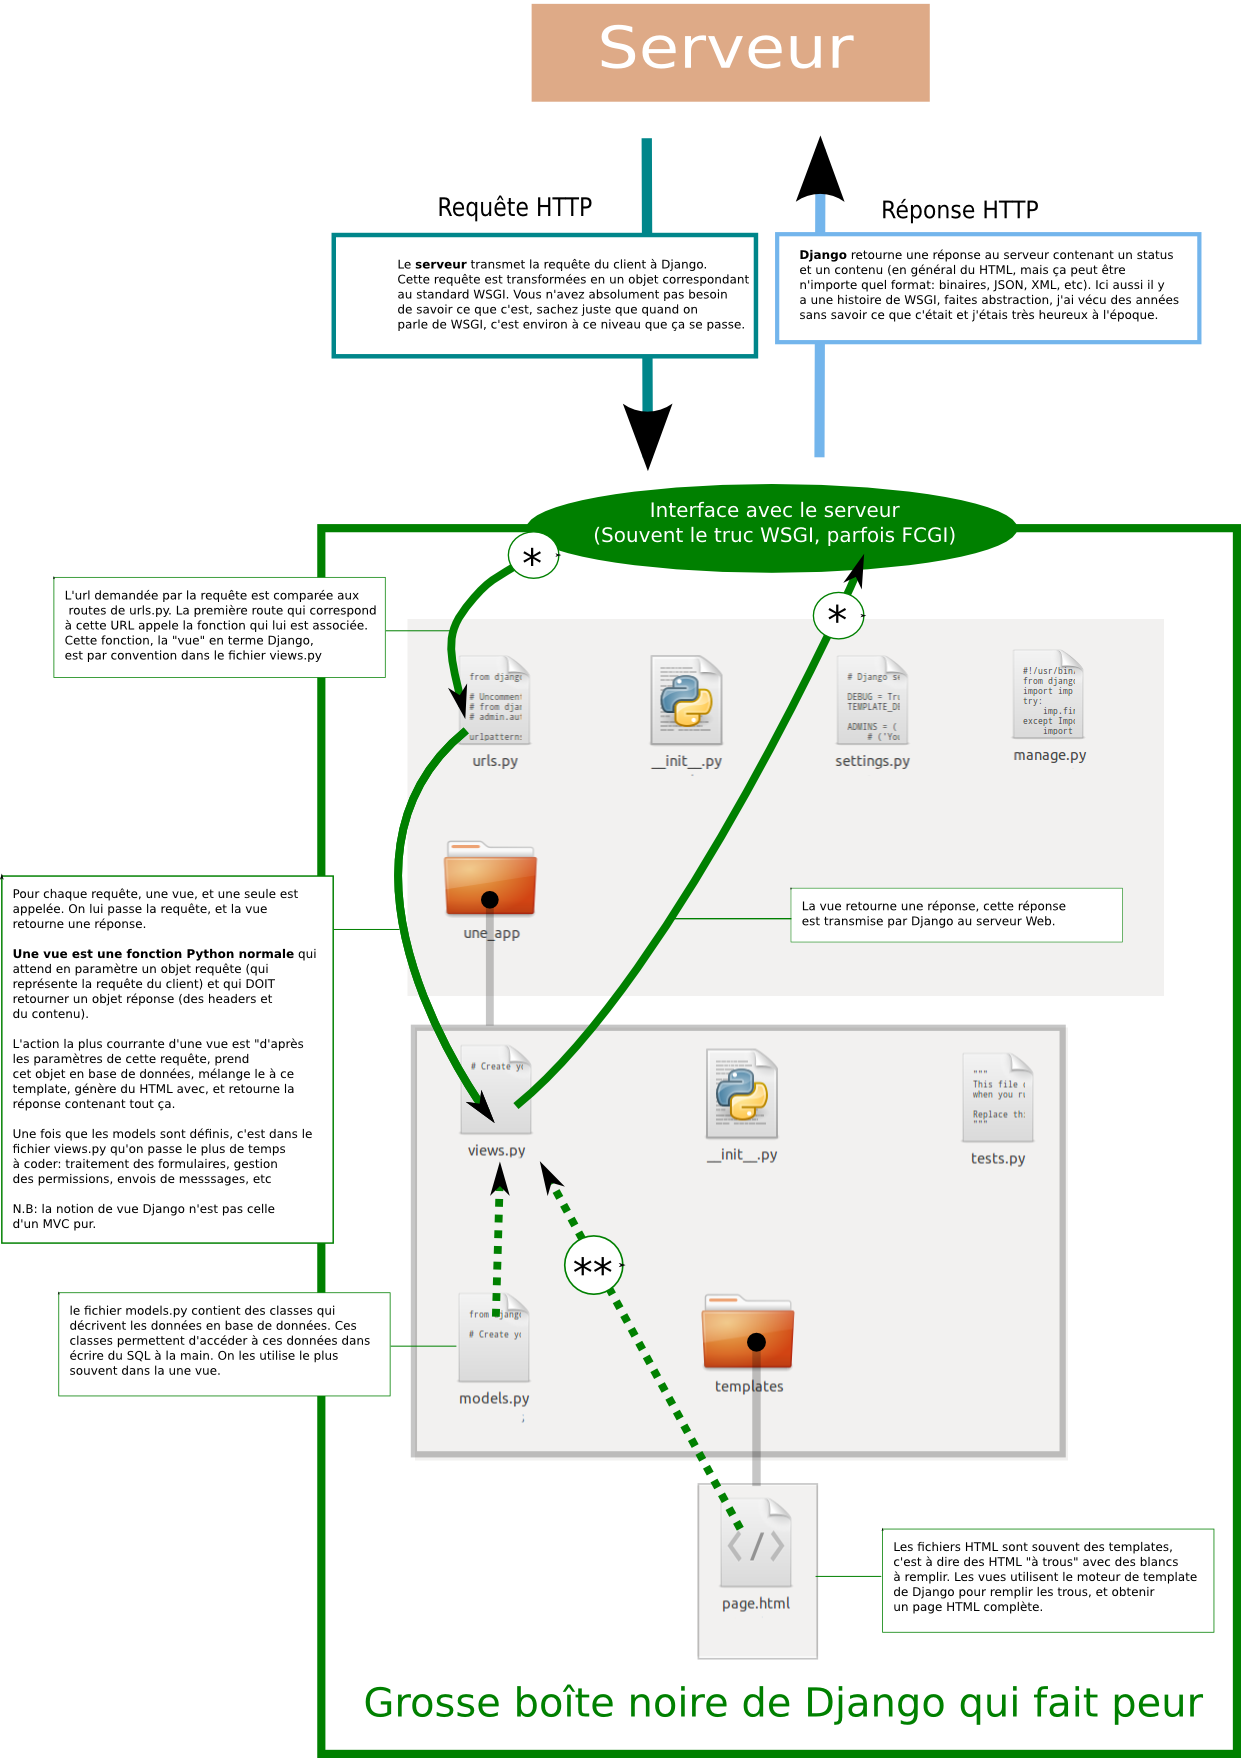
\includegraphics[scale=.18]{django.png}

    \footnotesize Source: http://sametmax.com/schema-de-fonctionnement-general-de-django/
\end{center}
\end{frame}

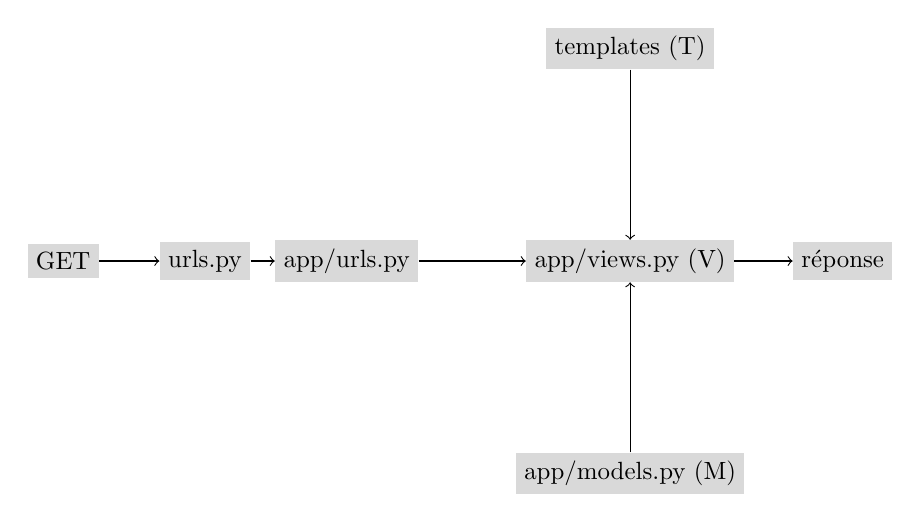
\begin{tikzpicture}[scale=.9, transform shape]
\tikzstyle{every node} = [fill=gray!30]
\node (a) at (0, 0) {GET};
\node (k) at (2, 0) {urls.py};
\node (b) at (4, 0) {app/urls.py};
\node (c) at (8, 0) {app/views.py (V)};
\node (e) at (8, 3) {templates (T)};
\node (f) at (8, -3) {app/models.py (M)};
\node (d) at (11, 0) {réponse};
\foreach \from/\to in {a/k, k/b, b/c, c/d, e/c, f/c}
\draw [->] (\from) -- (\to);
\end{tikzpicture}

\begin{frame}[fragile]{Exercice}
    Migrer dans une Django app.
\end{frame}

\begin{frame}[fragile]{}
\begin{LARGE}
\begin{center}
Avancé
\end{center}
\end{LARGE}
\end{frame}

\begin{frame}[fragile]{Arguments nomées dans les urls}

    Donner un nom aux arguments dans les urls:
\begin{Verbatim}[commandchars=\\\{\}]
    \PY{n}{url}\PY{p}{(}\PY{l+s}{r'}\PY{l+s}{\PYZca{}post/(?P\PYZlt{}post\PYZus{}id\PYZgt{}}\PY{l+s}{\PYZbs{}}\PY{l+s}{d+)/\PYZdl{}}\PY{l+s}{'}\PY{p}{,} \PY{l+s}{'}\PY{l+s}{show\PYZus{}post}\PY{l+s}{'}\PY{p}{)}
\end{Verbatim}

    Utile pour les génériques views.
\end{frame}

\begin{frame}[fragile]{POST et GET dans les requests}
    Les arguments POST et GET sont mis dans des dictionnaires sur l'objet request:

\begin{Verbatim}[commandchars=\\\{\}]
    \PY{k}{def} \PY{n+nf}{vue}\PY{p}{(}\PY{n}{request}\PY{p}{)}\PY{p}{:}
        \PY{n}{request}\PY{o}{.}\PY{n}{POST}\PY{p}{[}\PY{l+s}{"}\PY{l+s}{clef}\PY{l+s}{"}\PY{p}{]}

    \PY{k}{def} \PY{n+nf}{autre\PYZus{}vue}\PY{p}{(}\PY{n}{request}\PY{p}{)}\PY{p}{:}
        \PY{n}{request}\PY{o}{.}\PY{n}{GET}\PY{o}{.}\PY{n}{get}\PY{p}{(}\PY{l+s}{"}\PY{l+s}{clef}\PY{l+s}{"}\PY{p}{)}
\end{Verbatim}

Il est préférable d'utiliser .get pour éviter une exception
\end{frame}

\begin{frame}[fragile]{Nomer ses urls}
Cela permet de faire des reverses pour avoir des urls relatives.
\begin{small}
\begin{Verbatim}[commandchars=\\\{\}]
    \PY{n}{url}\PY{p}{(}\PY{l+s}{r'}\PY{l+s}{\PYZca{}(?P\PYZlt{}post\PYZus{}id\PYZgt{}}\PY{l+s}{\PYZbs{}}\PY{l+s}{d+)/\PYZdl{}}\PY{l+s}{'}\PY{p}{,} \PY{l+s}{'}\PY{l+s}{show\PYZus{}post}\PY{l+s}{'}\PY{p}{,} \PY{n}{name}\PY{o}{=}\PY{l+s}{"}\PY{l+s}{nom_url}\PY{l+s}{"}\PY{p}{)}
\end{Verbatim}
\end{small}

Dans les templates:
\begin{footnotesize}
\begin{verbatim}
    <a href="">Lien vers un post</a>
\end{verbatim}
\end{footnotesize}

Dans une vue:
\begin{Verbatim}[commandchars=\\\{\}]
\PY{k+kn}{from} \PY{n+nn}{django.core.urlresolvers} \PY{k+kn}{import} \PY{n}{reverse}

\PY{k}{def} \PY{n+nf}{vue}\PY{p}{(}\PY{n}{request}\PY{p}{)}\PY{p}{:}
    \PY{o}{.}\PY{o}{.}\PY{o}{.}
    \PY{n}{reverse}\PY{p}{(}\PY{l+s}{'}\PY{l+s}{post}\PY{l+s}{'}\PY{p}{,} \PY{n}{args}\PY{o}{=}\PY{p}{[}\PY{n}{post}\PY{o}{.}\PY{n}{id}\PY{p}{]}\PY{p}{)}
    \PY{o}{.}\PY{o}{.}\PY{o}{.}
\end{Verbatim}

\end{frame}

\begin{frame}[fragile]{Avec un préfixe}
Pour éviter les conflits de noms entre apps:
\begin{footnotesize}
\begin{Verbatim}[commandchars=\\\{\}]
    \PY{p}{(}\PY{l+s}{r'}\PY{l+s}{\PYZca{}blog/}\PY{l+s}{'}\PY{p}{,} \PY{n}{include}\PY{p}{(}\PY{l+s}{'}\PY{l+s}{blog.urls}\PY{l+s}{'}\PY{p}{,} \PY{n}{namespace}\PY{o}{=}\PY{l+s}{'}\PY{l+s}{blog}\PY{l+s}{'}\PY{p}{,} \PY{n}{app\PYZus{}name}\PY{o}{=}\PY{l+s}{'}\PY{l+s}{blog}\PY{l+s}{'}\PY{p}{)}\PY{p}{)}\PY{p}{,}
\end{Verbatim}
\end{footnotesize}

Ce qui donne:
    \begin{verbatim}
    
    \end{verbatim}

Et pareil pour reverse:
\begin{Verbatim}[commandchars=\\\{\}]
    \PY{n}{reverse}\PY{p}{(}\PY{l+s}{"}\PY{l+s}{blog:post}\PY{l+s}{"}\PY{p}{,} \PY{n}{args}\PY{o}{=}\PY{p}{[}\PY{n}{post}\PY{o}{.}\PY{n}{id}\PY{p}{]}\PY{p}{)}
\end{Verbatim}

\end{frame}

\begin{frame}[fragile]{Template, filtres}
    Il existe toute une série de filtres applicables à une variable comme ça (marche aussi sur les variables dans les templatetags):
\begin{verbatim}
    {{ variable|filtre }}
\end{verbatim}

    Ils peuvent se chainer:
\begin{verbatim}
    {{ variable|filtre1:"argument"|filtre2:"autre argument"|filtre3 }}
\end{verbatim}

On y retrouve la plupart des opérations classiques sur les strings (cut, strip, slugify, lower, capitalize ...) et d'autres trucs plus spéciaux (slice par exemple).
\end{frame}

\begin{frame}[fragile]{Template, include}
    Le templatetag $include$ permet d'inclure un template dans un autre de la façon suivante:

    \begin{verbatim}
    
    \end{verbatim}

Remarque: préférez l'héritage pour les choses telles que les headers et les footers.
\end{frame}

\begin{frame}[fragile]{L'héritage de templates}
    Beaucoup plus intéressant que l'include:

    \vspace{3mm}$base.html$
\begin{footnotesize}
\begin{Verbatim}[commandchars=\\\{\}]
    \PY{n+nt}{\PYZlt{}html}\PY{n+nt}{\PYZgt{}}
        \PY{n+nt}{\PYZlt{}head}\PY{n+nt}{\PYZgt{}}
            ...
            \PYZob{}\PYZpc{} block head \PYZpc{}\PYZcb{}\PYZob{}\PYZpc{} endblock \PYZpc{}\PYZcb{}
        \PY{n+nt}{\PYZlt{}/head\PYZgt{}}
        \PY{n+nt}{\PYZlt{}body}\PY{n+nt}{\PYZgt{}}
            \PY{n+nt}{\PYZlt{}div} \PY{n+na}{id=}\PY{l+s}{"supermenu"}\PY{n+nt}{\PYZgt{}}
                ...
            \PY{n+nt}{\PYZlt{}/div\PYZgt{}}
            \PY{n+nt}{\PYZlt{}div} \PY{n+na}{class=}\PY{l+s}{"content"}\PY{n+nt}{\PYZgt{}}
            \PYZob{}\PYZpc{} block content \PYZpc{}\PYZcb{}
            \PYZob{}\PYZpc{} endblock \PYZpc{}\PYZcb{}
            \PY{n+nt}{\PYZlt{}/div\PYZgt{}}
        \PY{n+nt}{\PYZlt{}/body\PYZgt{}}
    \PY{n+nt}{\PYZlt{}/html\PYZgt{}}
\end{Verbatim}
\end{footnotesize}
\end{frame}

\begin{frame}[fragile]{L'héritage de templates}
    $example.html$
\begin{footnotesize}
\begin{Verbatim}[commandchars=\\\{\}]
    \PYZob{}\PYZpc{} extends "base.html" \PYZpc{}\PYZcb{}

    \PYZob{}\PYZpc{} block content \PYZpc{}\PYZcb{}
    \PY{n+nt}{\PYZlt{}p}\PY{n+nt}{\PYZgt{}}Super content\PY{n+nt}{\PYZlt{}/p\PYZgt{}}
    \PYZob{}\PYZpc{} endblock \PYZpc{}\PYZcb{}
\end{Verbatim}
\end{footnotesize}
\end{frame}

\begin{frame}[fragile]{Champs des modèles classiques}
    Il y a normalement tout ce qu'on peut trouver dans une bdd SQL classique et d'autres
    \begin{itemize}
        \item CharField
        \item TextField
        \item BooleanField
        \item DateField et DateTimeField
        \item EmailField
        \item URLField
        \item ForeignKeyField
        \item ManyToManyField(..., through="...")
        \item OneToOne
    \end{itemize}
Et les options classiques: null=True, blank=True, max\_lenght=255
\end{frame}

\begin{frame}[fragile]{\_\_unicode\_\_ pour un modèle}
    C'est intéressant de surcharger cette méthode, car c'est elle qui sera appelée par défaut dans un template (et ça rend la lecture dans un shell plus facile):

\begin{Verbatim}[commandchars=\\\{\}]
\PY{n}{Class} \PY{n}{Post}\PY{p}{(}\PY{n}{models}\PY{o}{.}\PY{n}{Model}\PY{p}{)}\PY{p}{:}
    \PY{o}{.}\PY{o}{.}\PY{o}{.}
    \PY{k}{def} \PY{n+nf}{\PYZus{}\PYZus{}unicode\PYZus{}\PYZus{}}\PY{p}{(}\PY{n+nb+bp}{self}\PY{p}{)}\PY{p}{:}
        \PY{k}{return} \PY{n+nb+bp}{self}\PY{o}{.}\PY{n}{title}
\end{Verbatim}

\begin{verbatim}
{{ post }} <- affiche le titre du post
\end{verbatim}
\end{frame}

\begin{frame}[fragile]{Les reverses des modèles}
    Si vous faites des relations entre modèles avec des foreigns key, Django crée automatiquement des méthodes pour vous aider.

\vspace{3mm}
\pause
    Par exemple si vous avez un modèle Post et un modèle Comment qui a une foreign key vert Post, vous pouvez faire:

\begin{Verbatim}[commandchars=\\\{\}]
    \PY{n}{post} \PY{o}{=} \PY{n}{Post}\PY{o}{.}\PY{n}{objects}\PY{o}{.}\PY{n}{get}\PY{p}{(}\PY{n+nb}{id}\PY{o}{=}\PY{l+m+mi}{1}\PY{p}{)}
    \PY{n}{post}\PY{o}{.}\PY{n}{comment\PYZus{}set}\PY{o}{.}\PY{n}{all}\PY{p}{(}\PY{p}{)}
\end{Verbatim}

    $model\_set$ est un manager comme $objects$ et vous pouvez faire tout ce que vous pouvez faire avec objects dessus.
\end{frame}

\begin{frame}[fragile]{get\_object\_or\_404}
    Un shortcut sympa:

\begin{Verbatim}[commandchars=\\\{\}]
    \PY{k+kn}{from} \PY{n+nn}{django.shortcuts} \PY{k+kn}{import} \PY{n}{get\PYZus{}object\PYZus{}or\PYZus{}404}

    \PY{k}{def} \PY{n+nf}{vue}\PY{p}{(}\PY{n}{request}\PY{p}{)}\PY{p}{:}
        \PY{n}{post} \PY{o}{=} \PY{n}{get\PYZus{}object\PYZus{}or\PYZus{}404}\PY{p}{(}\PY{n}{Post}\PY{p}{,} \PY{n+nb}{id}\PY{o}{=}\PY{l+m+mi}{1}\PY{p}{)}
\end{Verbatim}


\pause
Remplace:

\begin{Verbatim}[commandchars=\\\{\}]
    \PY{k+kn}{from} \PY{n+nn}{django.http} \PY{k+kn}{import} \PY{n}{Http404}

    \PY{k}{def} \PY{n+nf}{my\PYZus{}view}\PY{p}{(}\PY{n}{request}\PY{p}{)}\PY{p}{:}
        \PY{k}{try}\PY{p}{:}
            \PY{n}{post} \PY{o}{=} \PY{n}{Post}\PY{o}{.}\PY{n}{objects}\PY{o}{.}\PY{n}{get}\PY{p}{(}\PY{n}{pk}\PY{o}{=}\PY{l+m+mi}{1}\PY{p}{)}
        \PY{k}{except} \PY{n}{Post}\PY{o}{.}\PY{n}{DoesNotExist}\PY{p}{:}
            \PY{k}{raise} \PY{n}{Http404}
\end{Verbatim}

\end{frame}

\begin{frame}[fragile]{Les génériques views}
    Très pratique mais un peu difficile à comprendre, y en a pour plusieurs types de choses:
    \begin{itemize}
        \item afficher le résultat d'un select
        \item afficher un objet
        \item créer un nouvel objet
        \item updater un objet
        \item supprimer un objet
        \item afficher un template et afficher par rapport à un type de date
    \end{itemize}
\end{frame}

\begin{frame}[fragile]{Les génériques views}
Ex: pour du listing et le detail (nom des templates \begin{bf}important\end{bf}):
\begin{footnotesize}
\begin{Verbatim}[commandchars=\\\{\}]
\PY{k+kn}{from} \PY{n+nn}{django.views.generic} \PY{k+kn}{import} \PY{n}{ListModel}

\PY{n}{urlpatterns} \PY{o}{=} \PY{n}{patterns}\PY{p}{(}\PY{l+s}{'}\PY{l+s}{'}\PY{p}{,}
    \PY{n}{url}\PY{p}{(}\PY{l+s}{r'}\PY{l+s}{\PYZca{}\PYZdl{}}\PY{l+s}{'}\PY{p}{,} \PY{n}{ListModel}\PY{o}{.}\PY{n}{as\PYZus{}view}\PY{p}{(}\PY{n}{model}\PY{o}{=}\PY{n}{Post}\PY{p}{)}\PY{p}{)}\PY{p}{,}
    \PY{n}{url}\PY{p}{(}\PY{l+s}{r'}\PY{l+s}{\PYZca{}post/(?P\PYZlt{}pk\PYZgt{}}\PY{l+s}{\PYZbs{}}\PY{l+s}{d+)/\PYZdl{}}\PY{l+s}{'}\PY{p}{,} \PY{n}{DetailModel}\PY{o}{.}\PY{n}{as\PYZus{}view}\PY{p}{(}\PY{n}{model}\PY{o}{=}\PY{n}{Post}\PY{p}{)}\PY{p}{)}\PY{p}{,}
    \PY{p}{)}

\PY{c}{\PYZsh{} est l'equivalent de}

\PY{k}{def} \PY{n+nf}{list\PYZus{}posts}\PY{p}{(}\PY{n}{request}\PY{p}{)}\PY{p}{:}
    \PY{k}{return} \PY{n}{render}\PY{p}{(}\PY{n}{request}\PY{p}{,} \PY{l+s}{"}\PY{l+s}{blog/post\PYZus{}list.html}\PY{l+s}{"}\PY{p}{,}
                  \PY{p}{\PYZob{}}\PY{l+s}{"}\PY{l+s}{object\PYZus{}list}\PY{l+s}{"}\PY{p}{:} \PY{n}{Post}\PY{o}{.}\PY{n}{objects}\PY{o}{.}\PY{n}{all}\PY{p}{(}\PY{p}{)}\PY{p}{\PYZcb{}}\PY{p}{)}

\PY{k}{def} \PY{n+nf}{post\PYZus{}detail}\PY{p}{(}\PY{n}{request}\PY{p}{,} \PY{n}{pk}\PY{p}{)}\PY{p}{:}
    \PY{k}{return} \PY{n}{render}\PY{p}{(}\PY{n}{request}\PY{p}{,} \PY{l+s}{"}\PY{l+s}{blog/post\PYZus{}detail.html}\PY{l+s}{"}\PY{p}{,}
                  \PY{p}{\PYZob{}}\PY{l+s}{"}\PY{l+s}{object}\PY{l+s}{"}\PY{p}{:} \PY{n}{get\PYZus{}object\PYZus{}or\PYZus{}404}\PY{p}{(}\PY{n}{Post}\PY{p}{,} \PY{n}{pk}\PY{o}{=}\PY{n}{pk}\PY{p}{)}\PY{p}{\PYZcb{}}\PY{p}{)}

\PY{n}{urlpatterns} \PY{o}{=} \PY{n}{patterns}\PY{p}{(}\PY{l+s}{'}\PY{l+s}{'}\PY{p}{,}
    \PY{n}{url}\PY{p}{(}\PY{l+s}{r'}\PY{l+s}{\PYZca{}\PYZdl{}}\PY{l+s}{'}\PY{p}{,} \PY{n}{list\PYZus{}posts}\PY{p}{)}\PY{p}{,}
    \PY{n}{url}\PY{p}{(}\PY{l+s}{r'}\PY{l+s}{\PYZca{}post/(?P\PYZlt{}pk\PYZgt{}}\PY{l+s}{\PYZbs{}}\PY{l+s}{d+)/\PYZdl{}}\PY{l+s}{'}\PY{p}{,} \PY{n}{post\PYZus{}detail}\PY{p}{)}\PY{p}{,}
    \PY{p}{)}
\end{Verbatim}
\end{footnotesize}
\end{frame}

\begin{frame}[fragile]{Ce dont j'ai pas parlé}
    \begin{itemize}
        \item les fichiers statiques
        \item forms
        \item middleware
        \item templatestags customs et filters custom
        \item rss/atom
        \item commandes perso
        \item gestion des utilisateurs (login\_required)
        \item messages
        \item i18n
        \item fixtures
        \item trucs avancés dans les modèles (et les contexts managers (with))
        \item django-nonrel
        \item les trucs à savoir quand on passe en prod
        \item django-south
        \item le caching
        \item les django-apps cool
        \item et tout le reste
    \end{itemize}
\end{frame}

\begin{frame}[fragile]{}
\begin{center}
    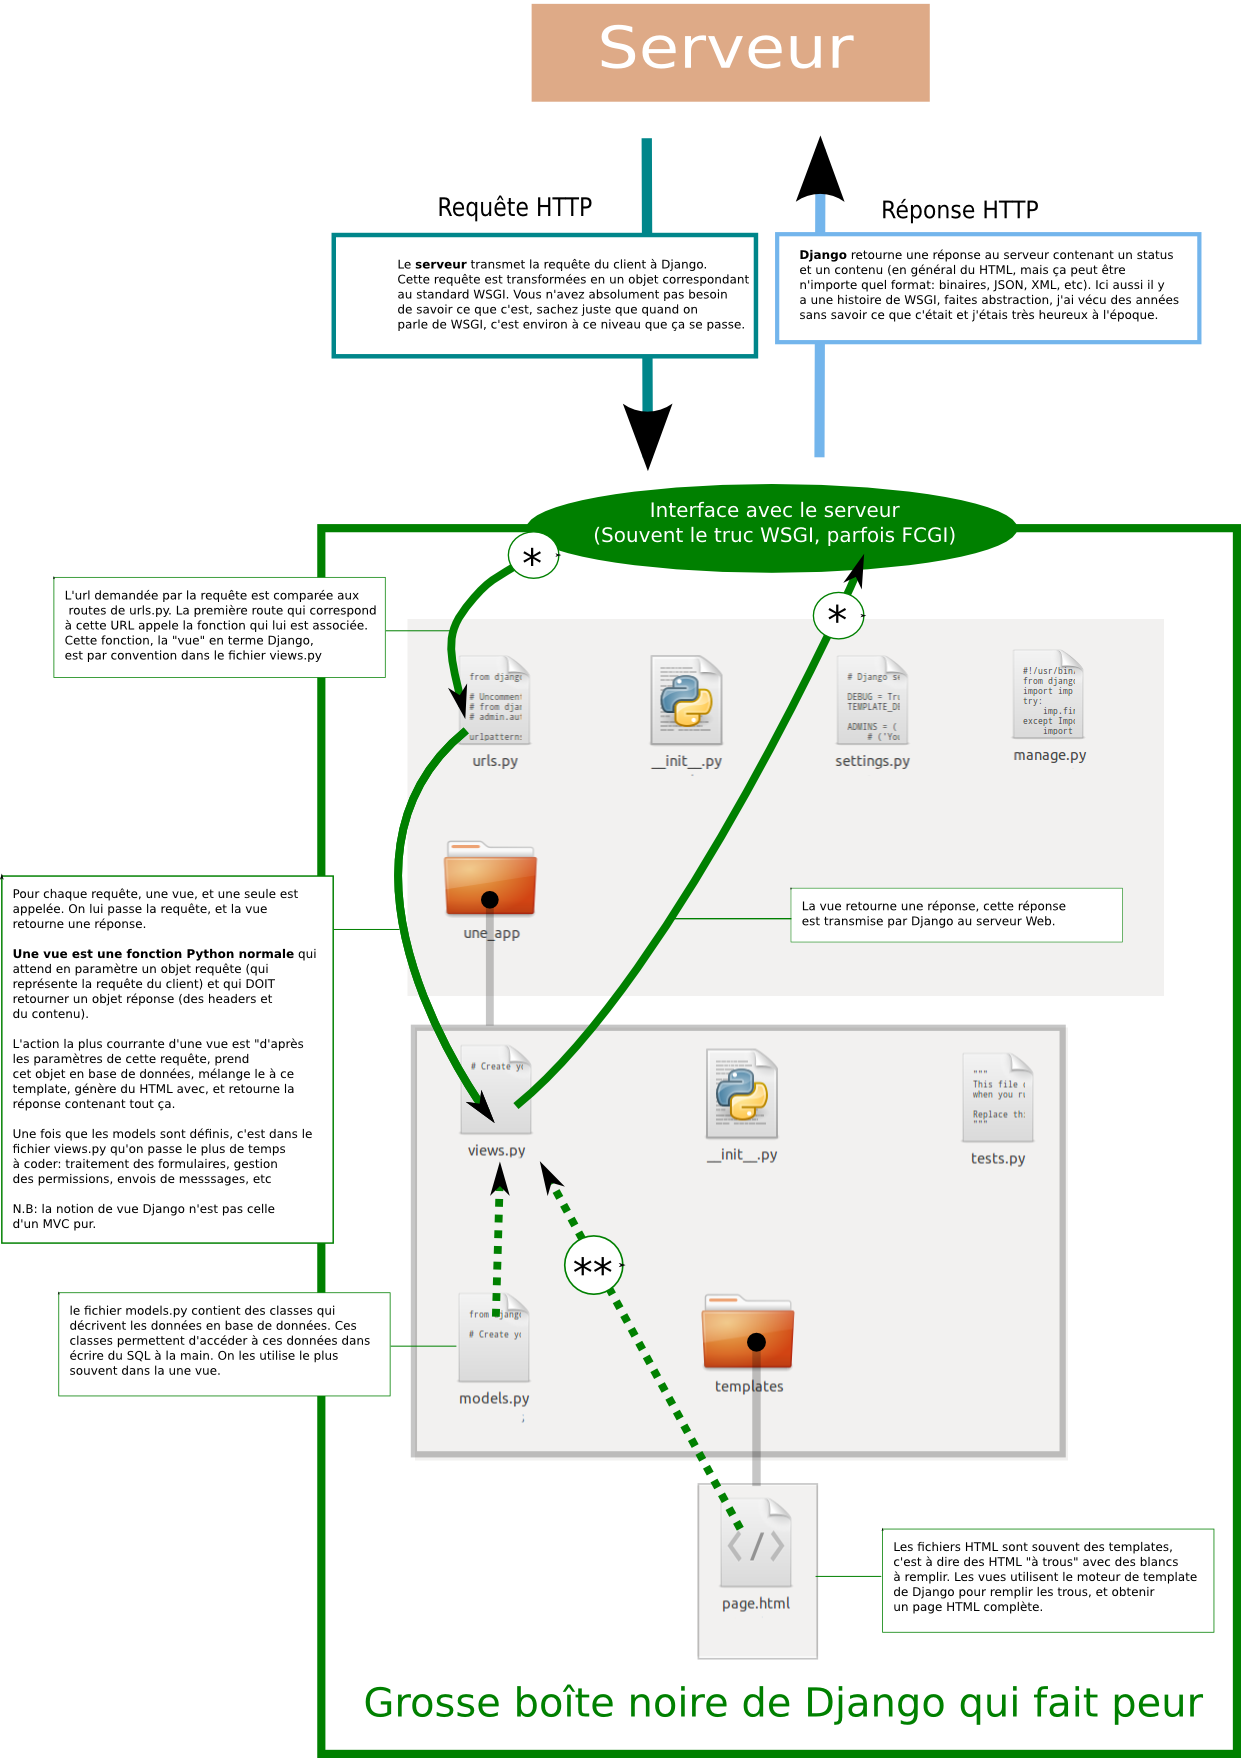
\includegraphics[scale=.18]{django.png}

    \footnotesize Source: http://sametmax.com/schema-de-fonctionnement-general-de-django/
\end{center}
\end{frame}

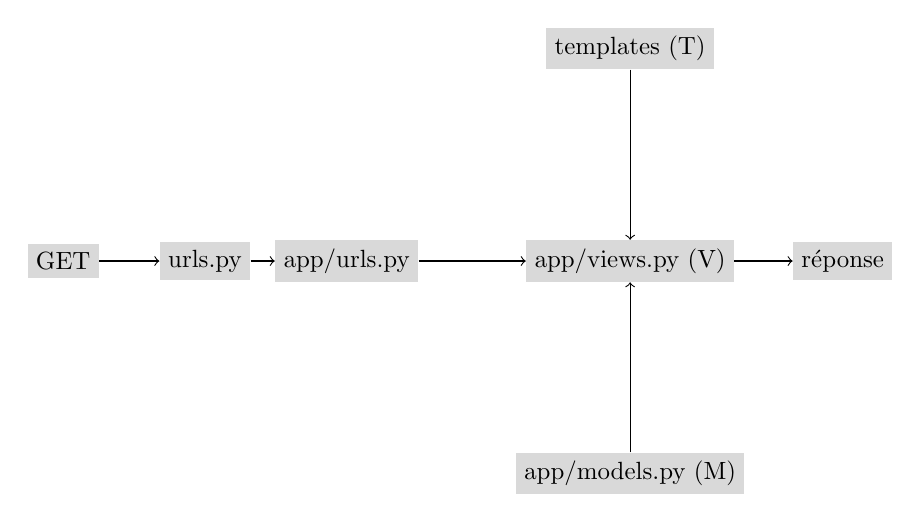
\begin{tikzpicture}[scale=.9, transform shape]
    MTV classique:
\tikzstyle{every node} = [fill=gray!30]
\node (a) at (0, 0) {GET};
\node (k) at (2, 0) {urls.py};
\node (b) at (4, 0) {app/urls.py};
\node (c) at (8, 0) {app/views.py (V)};
\node (e) at (8, 3) {templates (T)};
\node (f) at (8, -3) {app/models.py (M)};
\node (d) at (11, 0) {réponse};
\foreach \from/\to in {a/k, k/b, b/c, c/d, e/c, f/c}
\draw [->] (\from) -- (\to);
\end{tikzpicture}

\begin{frame}[fragile]{}
\begin{LARGE}
\begin{center}
Jquery
\end{center}
\end{LARGE}
\end{frame}

\begin{frame}[fragile]{Présentation}
    \begin{itemize}
        \item javascript web pour les humains\pause
        \item still javascript ...\pause
        \item surtout intéressant pour rendre une page dynamique\pause
        \item et faire de l'AJAX (en gros du POST/GET http sans recharger la page)\pause
        \item firebug (ou le brol buildin de chrome) sera votre compagnon d'infortune\pause
        \item utilisé par p402\pause
        \item surtout vous montrer le principe\pause
        \item pas oublier que c'est executé par le naviguateur de l'utilisateur qui peut le modifier (ou en empêcher son execution)
    \end{itemize}
\end{frame}

\begin{frame}[fragile]{Playground}
    Template avec lequel on va jouer:
\begin{small}
\begin{Verbatim}[commandchars=\\\{\}]
\PY{c+cp}{\PYZlt{}!doctype html\PYZgt{}}
\PY{n+nt}{\PYZlt{}html}\PY{n+nt}{\PYZgt{}}
  \PY{n+nt}{\PYZlt{}head}\PY{n+nt}{\PYZgt{}}
    \PY{n+nt}{\PYZlt{}meta} \PY{n+na}{charset=}\PY{l+s}{"utf-8"}\PY{n+nt}{\PYZgt{}}
    \PY{n+nt}{\PYZlt{}title}\PY{n+nt}{\PYZgt{}}Demo\PY{n+nt}{\PYZlt{}/title\PYZgt{}}
    \PY{n+nt}{\PYZlt{}style}\PY{n+nt}{\PYZgt{}}
        \PY{n+nc}{.test} \PY{p}{\PYZob{}} \PY{k}{font-weight}\PY{o}{:} \PY{k}{bold}\PY{p}{;} \PY{p}{\PYZcb{}}
    \PY{n+nt}{\PYZlt{}/style\PYZgt{}}
  \PY{n+nt}{\PYZlt{}/head\PYZgt{}}
  \PY{n+nt}{\PYZlt{}body}\PY{n+nt}{\PYZgt{}}
    \PY{n+nt}{\PYZlt{}script }\PY{n+na}{src=}\PY{l+s}{"jquery-1.7.2.min.js"}\PY{n+nt}{\PYZgt{}}\PY{n+nt}{\PYZlt{}/script\PYZgt{}}
    \PY{n+nt}{\PYZlt{}script}\PY{n+nt}{\PYZgt{}}
       \PY{n+nx}{\PYZdl{}}\PY{p}{(}\PY{n+nb}{document}\PY{p}{)}\PY{p}{.}\PY{n+nx}{ready}\PY{p}{(}\PY{k+kd}{function}\PY{p}{(}\PY{p}{)}\PY{p}{\PYZob{}}
            // on met le code jquery ici
       \PY{p}{\PYZcb{}}\PY{p}{)}\PY{p}{;}
   \PY{n+nt}{\PYZlt{}/script\PYZgt{}}
  \PY{n+nt}{\PYZlt{}/body\PYZgt{}}
\PY{n+nt}{\PYZlt{}/html\PYZgt{}}
\end{Verbatim}
\end{small}
\end{frame}

\begin{frame}[fragile]{Principe}
    Les uses cases de base sont assez simples:
    \begin{itemize}
        \item sélectionner un élément du DOM (l'arbre html) et le modifier
        \item selectionner un élément du DOM et lui attacher un événement
        \item faire une requète (POST/GET) et potentiellement utiliser le coder de retour
    \end{itemize}
\end{frame}

\begin{frame}[fragile]{Selectionner}
    C'est relativement simple:

\begin{Verbatim}[commandchars=\\\{\}]
\PY{n+nx}{\PYZdl{}}\PY{p}{(}\PY{l+s+s2}{"ici on met la query"}\PY{p}{)}
\end{Verbatim}
    Ça ressemble à du xpath simplifié:

    \begin{footnotesize}
\begin{Verbatim}[commandchars=\\\{\}]
\PY{n+nx}{\PYZdl{}}\PY{p}{(}\PY{l+s+s2}{"p"}\PY{p}{)} \PY{c+c1}{// tous les elements \PYZlt{}p\PYZgt{}}
\PY{n+nx}{\PYZdl{}}\PY{p}{(}\PY{l+s+s2}{"p.nom\PYZus{}de\PYZus{}class"}\PY{p}{)} \PY{c+c1}{// tous les elements \PYZlt{}p class="nom\PYZus{}de\PYZus{}class"\PYZgt{}}
\PY{n+nx}{\PYZdl{}}\PY{p}{(}\PY{l+s+s2}{"p\PYZsh{}pouet"}\PY{p}{)} \PY{c+c1}{// tous les elements \PYZlt{}p id="pouet"\PYZgt{}}
             \PY{c+c1}{// (normalement y en a qu'un seul sur du bon html)}
\PY{n+nx}{\PYZdl{}}\PY{p}{(}\PY{l+s+s2}{".nom\PYZus{}de\PYZus{}class"}\PY{p}{)} \PY{c+c1}{// tous les elements ayant la class correspondante}
\PY{n+nx}{\PYZdl{}}\PY{p}{(}\PY{l+s+s2}{"\PYZsh{}pouet"}\PY{p}{)} \PY{c+c1}{// tous les elements avec cet id}
\end{Verbatim}
\end{footnotesize}
\end{frame}

\begin{frame}[fragile]{Exemple}
    Exemple idiot (à tester si ça vous amuse):
\begin{Verbatim}[commandchars=\\\{\}]
    \PY{n+nx}{\PYZdl{}}\PY{p}{(}\PY{l+s+s2}{"p"}\PY{p}{)}\PY{p}{.}\PY{n+nx}{remove}\PY{p}{(}\PY{p}{)}\PY{p}{;}
    \PY{c+c1}{// va supprimer tous les \PYZlt{}p\PYZgt{} de votre page}
\end{Verbatim}
    Autre:
\begin{Verbatim}[commandchars=\\\{\}]
    \PY{n+nx}{\PYZdl{}}\PY{p}{(}\PY{l+s+s2}{"p"}\PY{p}{)}\PY{p}{.}\PY{n+nx}{text}\PY{p}{(}\PY{l+s+s2}{"Atchoum"}\PY{p}{)}\PY{p}{;}
\end{Verbatim}
\end{frame}

\begin{frame}[fragile]{Événements}
    Exemple, dans l'html:
\begin{Verbatim}[commandchars=\\\{\}]
    \PY{n+nt}{\PYZlt{}p}\PY{n+nt}{\PYZgt{}}\PY{n+nt}{\PYZlt{}a} \PY{n+na}{href=}\PY{l+s}{"\PYZsh{}"} \PY{n+na}{id=}\PY{l+s}{"hide"}\PY{n+nt}{\PYZgt{}}hide\PY{n+nt}{\PYZlt{}/a\PYZgt{}} -
       \PY{n+nt}{\PYZlt{}a} \PY{n+na}{href=}\PY{l+s}{"\PYZsh{}"} \PY{n+na}{id=}\PY{l+s}{"show"}\PY{n+nt}{\PYZgt{}}show\PY{n+nt}{\PYZlt{}/a\PYZgt{}}\PY{n+nt}{\PYZlt{}/p\PYZgt{}}

    \PY{n+nt}{\PYZlt{}p} \PY{n+na}{id=}\PY{l+s}{"pouet"}\PY{n+nt}{\PYZgt{}}Foobarbaz\PY{n+nt}{\PYZlt{}/p\PYZgt{}}
\end{Verbatim}
    Dans la partie jquery:
\begin{Verbatim}[commandchars=\\\{\}]
    \PY{n+nx}{\PYZdl{}}\PY{p}{(}\PY{l+s+s2}{"\PYZsh{}hide"}\PY{p}{)}\PY{p}{.}\PY{n+nx}{click}\PY{p}{(}\PY{k+kd}{function}\PY{p}{(}\PY{n+nx}{event}\PY{p}{)} \PY{p}{\PYZob{}}
        \PY{n+nx}{\PYZdl{}}\PY{p}{(}\PY{l+s+s2}{"\PYZsh{}pouet"}\PY{p}{)}\PY{p}{.}\PY{n+nx}{hide}\PY{p}{(}\PY{l+s+s2}{"slow"}\PY{p}{)}\PY{p}{;}
    \PY{p}{\PYZcb{}}\PY{p}{)}\PY{p}{;}
    \PY{n+nx}{\PYZdl{}}\PY{p}{(}\PY{l+s+s2}{"\PYZsh{}show"}\PY{p}{)}\PY{p}{.}\PY{n+nx}{click}\PY{p}{(}\PY{k+kd}{function}\PY{p}{(}\PY{n+nx}{event}\PY{p}{)} \PY{p}{\PYZob{}}
        \PY{n+nx}{\PYZdl{}}\PY{p}{(}\PY{l+s+s2}{"\PYZsh{}pouet"}\PY{p}{)}\PY{p}{.}\PY{n+nx}{show}\PY{p}{(}\PY{l+s+s2}{"slow"}\PY{p}{)}\PY{p}{;}
    \PY{p}{\PYZcb{}}\PY{p}{)}\PY{p}{;}
\end{Verbatim}
    Exemple réel: un menu déroulant.
\end{frame}

\begin{frame}[fragile]{AJAX: GET}
    GET (remarque, l'ajax n'est permis que sur le domaine où s'excecute le code):
\begin{Verbatim}[commandchars=\\\{\}]
    \PY{n+nx}{\PYZdl{}}\PY{p}{.}\PY{n+nx}{get}\PY{p}{(}\PY{l+s+s2}{"/url/"}\PY{p}{,} \PY{k+kd}{function}\PY{p}{(}\PY{n+nx}{data}\PY{p}{)} \PY{p}{\PYZob{}}
        \PY{n+nx}{\PYZdl{}}\PY{p}{(}\PY{l+s+s2}{"\PYZsh{}pouet"}\PY{p}{)}\PY{p}{.}\PY{n+nx}{html}\PY{p}{(}\PY{n+nx}{data}\PY{p}{)}\PY{p}{;}
    \PY{p}{\PYZcb{}}\PY{p}{)}\PY{p}{;}
\end{Verbatim}
    Pratique pour le chargement asynchrone du contenu d'une page.
\end{frame}

\begin{frame}[fragile]{AJAX: POST}
    POST similaire au GET:

    \begin{footnotesize}
\begin{Verbatim}[commandchars=\\\{\}]
    \PY{n+nx}{\PYZdl{}}\PY{p}{.}\PY{n+nx}{post}\PY{p}{(}\PY{l+s+s2}{"/url/"}\PY{p}{,} \PY{k+kd}{function}\PY{p}{(}\PY{n+nx}{data}\PY{p}{)} \PY{p}{\PYZob{}}
        \PY{c+c1}{// ...}
    \PY{p}{\PYZcb{}}\PY{p}{)}\PY{p}{;}
\end{Verbatim}
\end{footnotesize}

    On peut lui donner des données (au GET aussi):

    \begin{footnotesize}
\begin{Verbatim}[commandchars=\\\{\}]
    \PY{n+nx}{\PYZdl{}}\PY{p}{.}\PY{n+nx}{post}\PY{p}{(}\PY{l+s+s2}{"/url/"}\PY{p}{,} \PY{p}{\PYZob{}}\PY{n+nx}{name}\PY{o}{:} \PY{l+s+s2}{"pouet"}\PY{p}{,} \PY{n+nx}{password}\PY{o}{:} \PY{l+s+s2}{"toto"}\PY{p}{\PYZcb{}}\PY{p}{,} \PY{k+kd}{function}\PY{p}{(}\PY{n+nx}{data}\PY{p}{)} \PY{p}{\PYZob{}}
        \PY{c+c1}{// ...}
    \PY{p}{\PYZcb{}}\PY{p}{)}\PY{p}{;}
\end{Verbatim}
\end{footnotesize}

    Ou le contenu d'une form (au GET aussi):
    \begin{footnotesize}
\begin{Verbatim}[commandchars=\\\{\}]
    \PY{n+nx}{\PYZdl{}}\PY{p}{.}\PY{n+nx}{post}\PY{p}{(}\PY{l+s+s2}{"/url/"}\PY{p}{,} \PY{n+nx}{\PYZdl{}}\PY{p}{(}\PY{l+s+s2}{"\PYZsh{}my\PYZus{}form"}\PY{p}{)}\PY{p}{.}\PY{n+nx}{serialize}\PY{p}{(}\PY{p}{)}\PY{p}{,} \PY{k+kd}{function}\PY{p}{(}\PY{n+nx}{data}\PY{p}{)} \PY{p}{\PYZob{}}
        \PY{c+c1}{// ...}
    \PY{p}{\PYZcb{}}\PY{p}{)}
\end{Verbatim}
\end{footnotesize}

    Remarques: le callback est optionnel et il existe un \$.getJSON qui marche pareil.
\end{frame}

\begin{frame}[fragile]{Remarques}
    Vous n'aurez pas besoin d'énormement plus, avec ça vous savez déjà faire énormement.

    \vspace{3mm}
    Je vous recommande vraiment d'apprendre à vous servir de firebug, de sa console et de la fenêtre qui permet de mettre des breakpoints.

    \vspace{3mm}
    L'unique commande à retenir pour la console:
    \begin{verbatim}
        console.dir(truc);
    \end{verbatim}
    Affiche les méthodes/attributs d'un objet.

    \vspace{3mm}
    Aussi intéressant de savoir que $console.log("foobar");$ affichera ça dans la console firebug.
\end{frame}

\begin{frame}[fragile]{}
\begin{LARGE}
\begin{center}
Faim. Questions/Remarques ?
\end{center}
\end{LARGE}
\end{frame}

\end{document}
